\documentclass{article}
\DeclareMathSizes{10}{10}{7}{7}
\usepackage{amsmath}
\usepackage{ amssymb }
\usepackage{tikz, graphicx}
\usepackage{geometry}
\usepackage[makeroom]{cancel}
\usepackage{ltablex}
\usepackage{calrsfs}
\DeclareMathAlphabet{\pazocal}{OMS}{zplm}{m}{n}
\usepackage[export]{adjustbox}
\usepackage[
backend=biber,
sorting=ynt
]{biblatex}
\addbibresource{references.bib}
\DeclareMathOperator{\sech}{sech}
\usepackage{subfig}
\usepackage[hidelinks]{hyperref}
\hypersetup{
    %colorlinks=true,
    %linkcolor=blue,
    %filecolor=magenta,      
    %urlcolor=blue,
    }
\usepackage{float}
\restylefloat{table}

\geometry{legalpaper, margin=0.7in}

\title{Noize net | Investigation into novel music genration using recurrent models}
\author{Liam Watson}
\begin{document}
\maketitle
\tableofcontents
\section{Abstract}
In this paper we give a brief overview of the structure, mathematics and reasoning used in neural networks and lead on to the structure and reasoning of recurrent models. We discuss RNN's as well as LSTM's and investigate their use in the generation of novel music. We discuss the various problems that arise when dealing with large, highly nonlinear data when using recurrent models and possible solutions. We discuss the implementation of an RNN and LSTM as well as the various hyper parameters that arise (the code can be found \href{https://github.com/Liam-Watson/NoizeNet/blob/main/code/FinalNoteBook.ipynb}{here}). We find that NoizeNet predictions converge to a constant value after few iterations and discuss potential solutions to this phenomenon. Overall find that novel music generation is feasible, however, it requires large input sequences and highly complex models. Given the lack of computational resources available in this work we cover data transformations and introduction of selective perturbations in order to improve results and find that they are ineffective.
\section{Introduction}
Artificial intelligence and machine learning has been a topic of much debate for many years in the theoretical space, however, in recent times advancements in computational power and theoretical models have brought these concepts into reality. The field of machine learning is broad with many types of models such as K Nearest Neighbors, decision trees, random forests and the topic of this paper neural networks. These different models have widely varying structural and behavioral properties but share the same defining principle, given some data the models have a scheme that they can use to learn how to better predict the some outcome from the input data data whether it be classification or time series prediction. These different models can be used to predict highly nonlinear data which before was infeasible with techniques like linear regression dominating the data analysis sphere. \\
In this paper we wish to investigate the feasibility of music generation using a class of neural network called an RNN which is specifically designed for time series data analysis.  
\section{Introduction to Neural networks}
\label{sec:intro}
Before we proceed to the more advanced recurrent neural network let us begin with an abbreviated coverage of neural networks and the concepts underpinning them. 
\subsection{Perceptron}
\label{sec:peceptrons}
The simplest unit of a neural network is a perceptron. A perceptron a model that takes input $\{x_1, x_2, ... ,x_n\}$ along with some weights for each input $\{w_1, w_2, .., w_N\}$. The output is a binary value determined by a step function centered at some value. \cite{Nielsen} We can adjust the center point of the step function using an additional input weight, the bias $b$ which can be seen in figure 1.
\begin{figure}[H]
\centering
\caption{Perceptron showing N input variables, N weights and a bias}
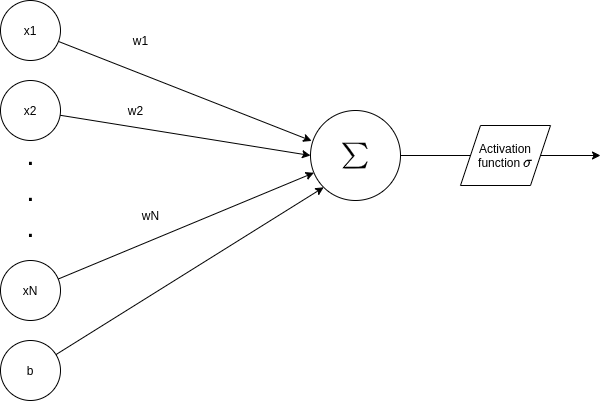
\includegraphics[scale=0.5]{peceptron.png}
\end{figure}
The output of the perceptron is calculated by point wise multiplying the weights (and bias) with the inputs, then passing the sum of the result through the step function. Mathematically this can be represented as a dot product of two vectors. 
\begin{align*}
\sigma \left(\begin{bmatrix}
&w_1 \\
&w_2 \\
&. \\
&. \\
&. \\
&w_n \\
&b \\
\end{bmatrix} 
\cdot 
\begin{bmatrix}
&x_1 \\
&x_2 \\
&. \\
&. \\
&. \\
&x_n \\
&1
\end{bmatrix}\right) = \sigma \left(w\cdot x\right)
\end{align*}
Given these inputs and bias we can adjust weights and bias to satisfy our desired output after summation and activation function (\ref{sec:activationfuncs}). 
More rigorously: Given some input $\{x_i\} \forall i\in \mathbb{Z^+}$ predict some $y=\sigma(W_i x_i)$ where $\sigma$ is the Heaviside step function. This model is only useful for very simple binary classification problems and has very little real world application in this form.

\pagebreak

\subsection{Multi layer perceptron network}
\label{sec:mlp}
We only begin to see the utility when we start connecting perceptrons together in a mesh much like neurons in the brain. In figure 2 we can see a depiction of this with weight values represented as line thickness (\autoref{fig:mlp}). 
\begin{figure}[H]
\caption{Image of a simple neural network architecture with 8 inputs two hidden layers and four output neurons. Image reproduced from Ref.\cite{3blue1brown}}
\label{fig:mlp}
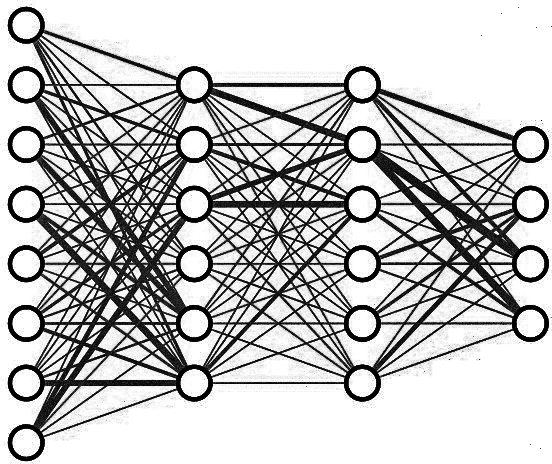
\includegraphics[scale=2]{nn.jpg}
\end{figure}
The mathematics here is similar to the single perceptron but, now the input values for any layer is determined by the previous layer. Mathematically this is readily represented as matrix vector multiplication. 
\begin{align*}
\sigma \left(\begin{bmatrix}
&w_{1,1} &w_{1,2} &.&.&. &w_{1,n} \\
&w_{2,1} &w_{2,2} &.&.&. &w_{2,n}  \\
&.&.&.&.&.&. \\
&. &.&.&.&.&.\\
&. &.&.&.&.&.\\
&w_{n,1} &w_{n,2} &.&.&. &w_{n,n}  \\
\end{bmatrix} 
\begin{bmatrix}
&x_1 \\
&x_2 \\
&. \\
&. \\
&. \\
&x_n \\
\end{bmatrix}
+
\begin{bmatrix}
&b_1 \\
&b_2 \\
&. \\
&. \\
&. \\
&b_n \\
\end{bmatrix}
\right) = \sigma \left(\textbf{W} \vec{x} + \vec{b}\right)
\end{align*}
Where the activation function is applied to each of the resulting vector elements. 
\subsection{Activation functions}
\label{sec:activationfuncs}
A binary step function is very limiting in terms of application to the real world, a continuous output would be far more useful for classification probabilities or in our case of this work, music generation. There are many functions that are used in the literature but here we give give a quick overview of the most common functions and their uses. The purpose of an activation function is to format the output of a perceptron into the desired range as the value could be any real value. We begin with the most elementary of these functions (excluding the identity function defined as $f(x) = x$). 
\begin{enumerate}
\item The binary step function \\
Definition:
\begin{align*}
f(x) = 
\begin{cases}
 1 & \text{if } x > 0 \\
 0 & \text{if } x \leq 0 \\
\end{cases}
\end{align*}
\begin{figure}[H]
\centering
\caption{A plot of the Heaviside step function}
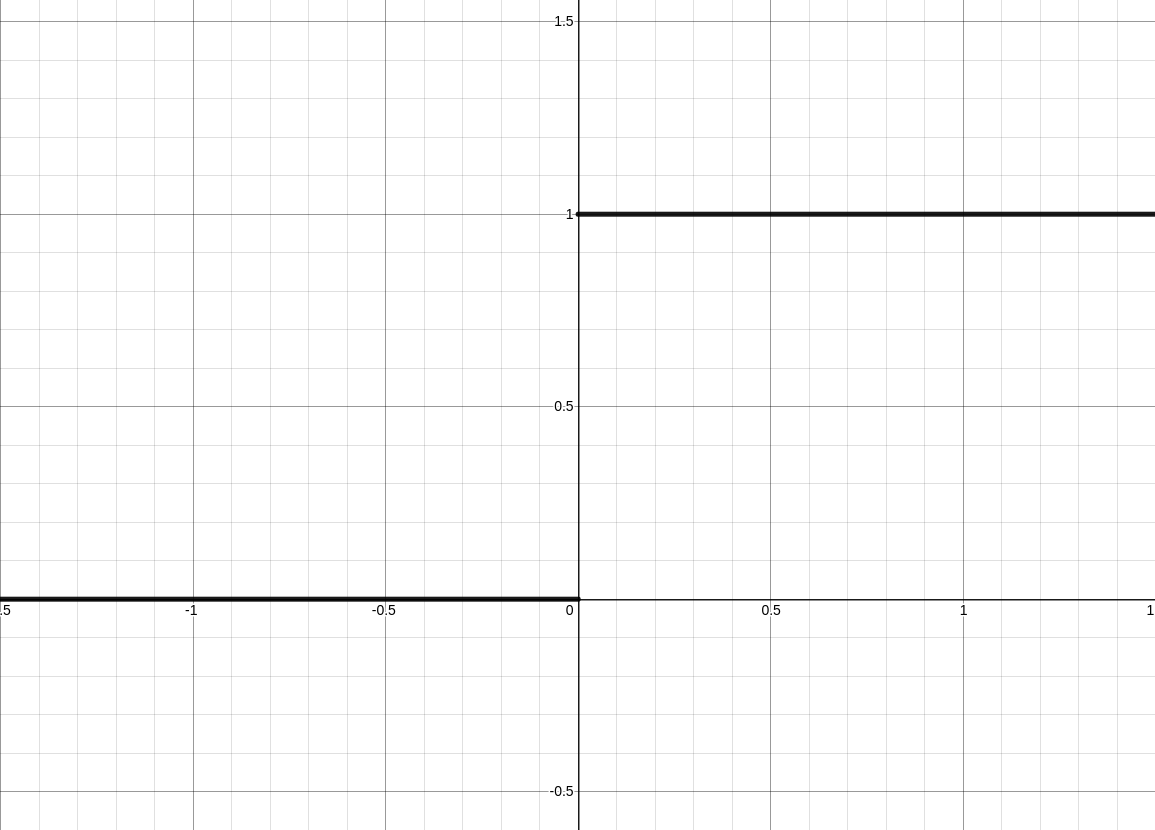
\includegraphics[scale=0.2]{heaviside.png}
\end{figure}
The binary step function is primarily used for true, false classification where the result is not a probability but a certainty. Beyond binary classification, this activation function has limited use in modern neural networks, however it should be noted that it is highly computationally efficient. 
\item Rectified Linear Unit (ReLU)\\
Definition: 
\begin{align*}
f(x) =
\begin{cases}
 0 & \text{if } x \leq 0 \\
 x & \text{if } x > 0 \\
\end{cases}
\end{align*}
\begin{figure}[H]
\centering
\caption{A plot of the ReLu function}
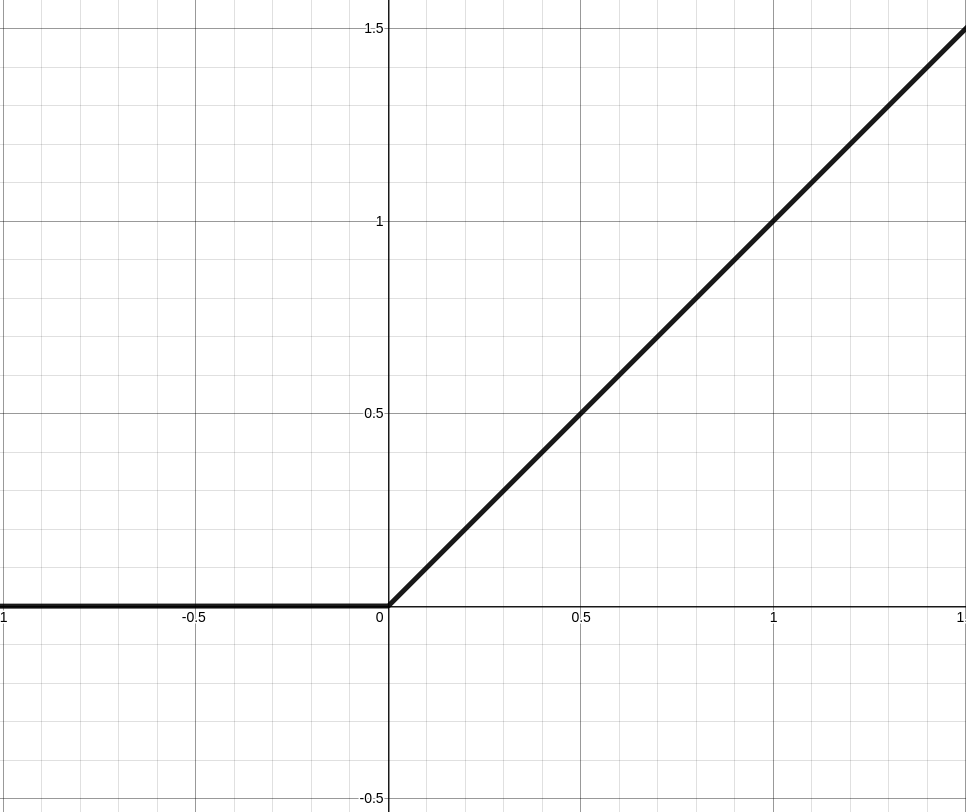
\includegraphics[scale=0.2]{relu.png}
\end{figure}
The ReLU Function finds much use despite its simplicity mostly due to its computational efficiency when compared to the more complex activation functions. ReLU reduces the input domain to only non-negative numbers which can be useful in cases where one wishes to disregard such values. 
\item Sigmoid \\
Definition: 
\begin{align*}
&f(x) = \frac{1}{1 + e^{-x}}
\end{align*}
\begin{figure}[H]
\centering
\caption{A plot of the sigmoid function}
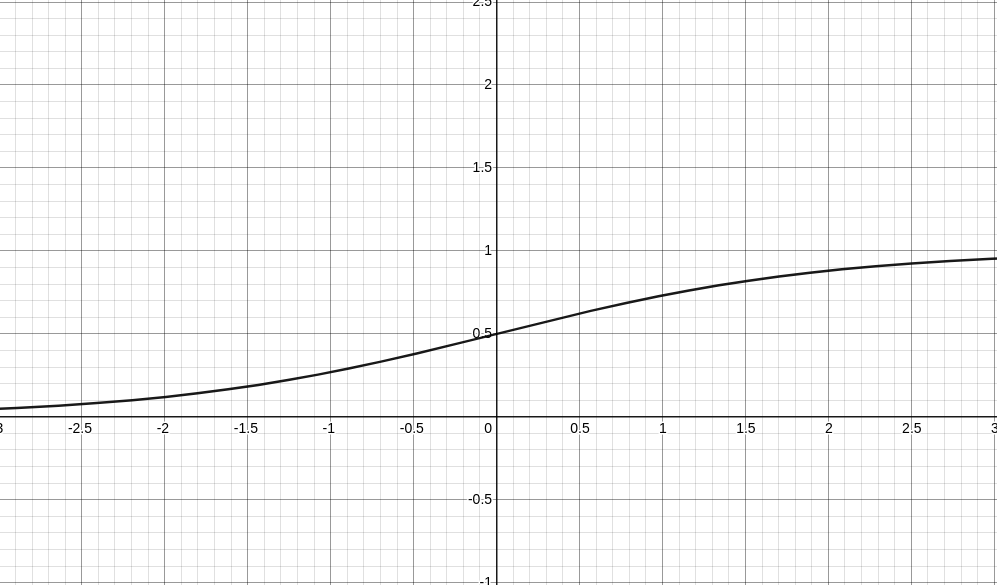
\includegraphics[scale=0.2]{sigmoid.png}
\end{figure}
The sigmoid function is widely used in classification problems where outputs are interpreted as probabilities. Additionally, the sigmoid finds use in more complex architectures such as the LSTM which we will discuss later. 
\item Hyperbolic Tangent\\
Definition:
\begin{align*}
f(x) = \frac{e^x - e^{-x}}{e^x + e^{-x}}
\end{align*}

\begin{figure}[H]
\centering
\caption{A plot of the $\tanh$ function}
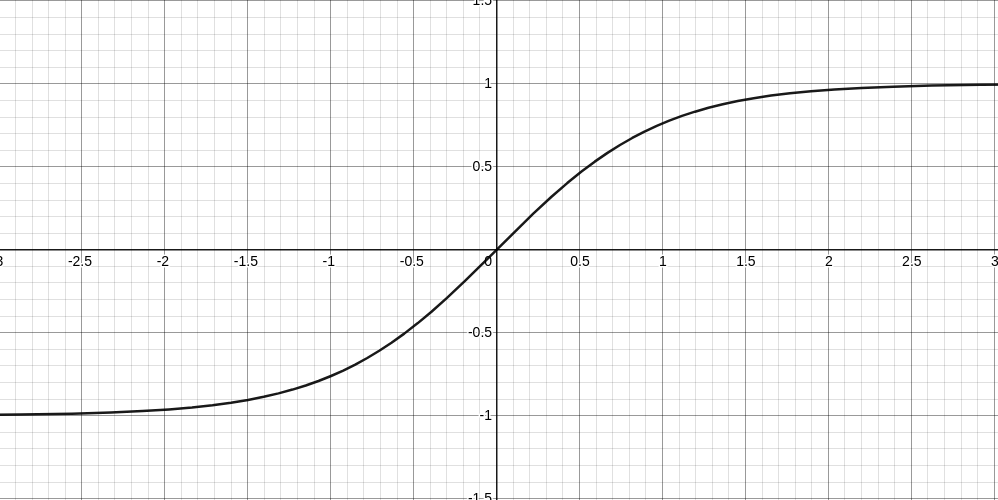
\includegraphics[scale=0.2]{tanh.png}
\end{figure}
This activation function is less widely used than the sigmoid function but is relevant in this paper as it is used in the architecture of an LSTM which we will cover later.
\end{enumerate}

\subsection{Feed forward}
\label{sec:forward}
Now we have covered how to calculate the activation's of each neuron in the network, we can now begin using the output. The output of the network is obtained during the feed forward stage of a network. The network will receive input's at the input neurons and propagate through all the network layers calculating activation's until the algorithm reaches the output layer. The activation's at the output layer are considered the network prediction. One can see why the phase is called feed forward, as the network propagates activation's "left to right", forward through the network. 
\subsection{Error functions (Loss functions)}
\label{sec:error}
Once we have output from the model, we need a metric for the error between the output prediction and ground truth, an error function. There are many error functions that appear in the literature, however, their use is often highly application dependent. In the case of music generation we are dealing with simple two dimensional time series data and as such the relevant error functions are elementary:
\begin{enumerate}
\item Mean Square Error (MSE)\\
This error function finds the average square difference between the predicted value and ground truth, defined as
\begin{align*}
MSE = \frac{\sum_{i=0}^N (y_i - y_i^\prime)^2}{N}
\end{align*}
Where $N$ is the number of output values, $y_i$ is the ground truth value and $y_i^\prime$ is the predicted value. \\
This loss function is favorable because of it's simplicity and computational efficiency. One should note that MSE can "amplify" large errors and "squash" small errors due to the square. Additionally, note that the direction of the error is also ignored.  MSE is considered the optimal error function as the functional calculates the relative distance between a prediction and ground truth. 
\item Mean absolute error \\
If one would not like to square the error in order to better capture small errors one can use the MAE function which shares many similar properties with the MSE function but depicts the difference between a prediction and the ground truth differently. 
\begin{align*}
MAE = \frac{\sum_{i=0}^N |y_i - y_i^\prime|}{N}
\end{align*}
\item Mean Bias error \\
If the application requires a signed error function the MBE error function could be applicable. However, one should note that positive and negative values may cancel each other out leading to unpredictable results in practice. 
\begin{align*}
MBE = \frac{\sum_{i=0}^N (y_i - y_i^\prime)}{N}
\end{align*}
\end{enumerate}
It should be noted that more complex loss functions are used for categorical data such as cross entropy loss or hinge Loss.

\subsection{Gradient decent}
\label{sec:gradientDecent}
Now we need a method to update the perceptron weights given some value for the error between some prediction and ground truth, for this we use gradient decent. There are many adaptions of gradient descent that aim to optimize its computational performance or over come some issue with converging to a poorly optimised solution such as fast gradient methods or momentum adapted gradient descent methods. \\
The aim of gradient descent is to iteratively optimize the perceptron weights in order to converge on a minimum loss (likely a local minimum) by taking steps in the direction of steepest descent, after many iterations we will find that the networks weights are well optimised for some goal. However we may find that a local minimum is not sufficient for our purposes and as such may need to employ some hyper parameter tuning such as changing the the step size we take or adding momentum in the hope that we converge to a more optimal solution.
\begin{figure}[H]
\centering
\caption{A plot of $f(x,y) = \sin(x) + \sin(y)$ with a path showing gradient decent steps}
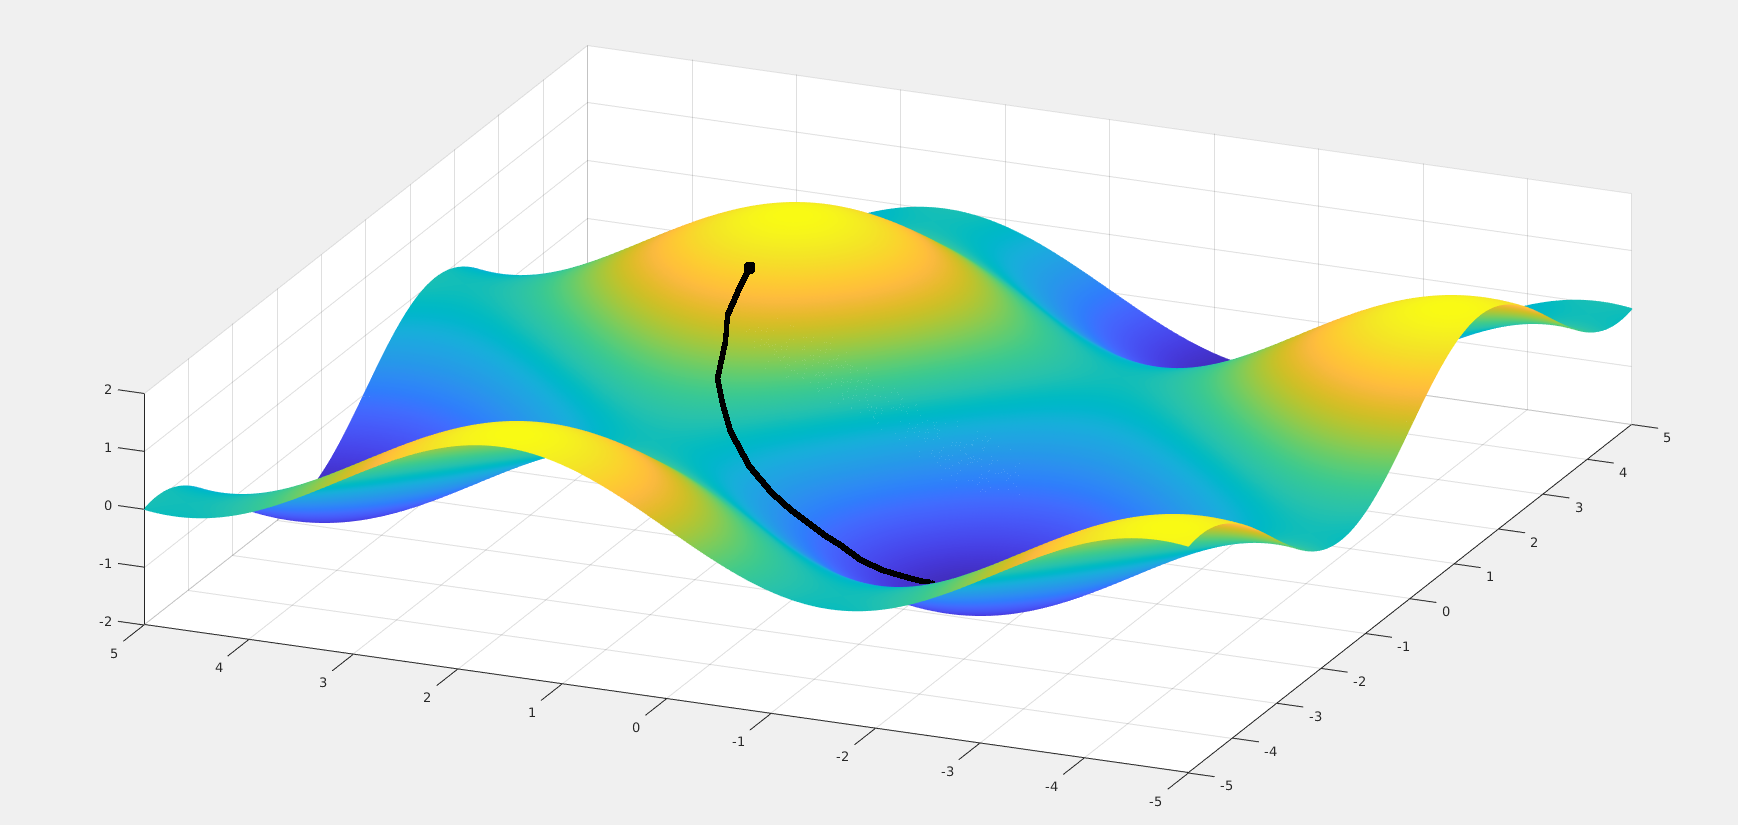
\includegraphics[scale=0.2]{mesh.png}
\end{figure}
Mathematically gradient descent is a simple optimization problem. First we must define the function that we wish to minimise. The cost is defined by some error function of the weights as discussed above where in the context of a neural network we sum the "difference"(absolute, squared or standard) between each of the output neurons and the ground truth value, then divide by the number of elements. So if we have some function that calculates the cost for all the weights over all the training data (a so called cost function $C(\mathbf{W})$) we can calculate the gradient $\nabla C$ and take a step in the opposite direction $-\nabla C$ as we wish to find the minimum of the cost function. By taking a step we mean that we adjust the weights and biases in order move in down the slope by some step size $\eta$. The magnitude and sign of the gradient of the cost function encodes the direction and magnitude of the amount that we must change the weights and biases in order to make the optimal change in their values. 
\subsection{Back propagation}
\label{sec:back}
Back propagation is the learning step for a model. Once we have completed the feed forward step and calculated the error we need to travel back through the network and adjust the weights and biases in order to optimize the model, decrease the cost. We change the weights and bias at each layer recursively according to the gradient descent step.  There is much more to cover here - excluded for brevity - but this is the general idea. 
\section{Introduction to Recurrent Neural Networks}
\label{sec:intoRNNs}
When using neural networks for time series data prediction, some semblance of memory is required for successive predictions. Unfortunately standard multi-layer perceptron and convolutional neural networks tend to lose this information quickly as they train due to the vanishing gradient problem. RNNs seek to resolve this by using past states in a current prediction. More advanced models construct hand crafted compositions of so called "gates" that can incorporate prior information for successive predictions in more complex ways. 

\subsection{RNN concepts}
\label{sec:RNNS}
RNNs are designed specifically to learn from sequences of data by passing the hidden state from one step in the sequence to the next step in the sequence, combined with the input. This gives RNNs the ability to predict sequences of values using knowledge of past state as well as current state. 
\begin{figure}[H]
\centering
\caption{RNN basic architecture}
\label{fig:RNN}
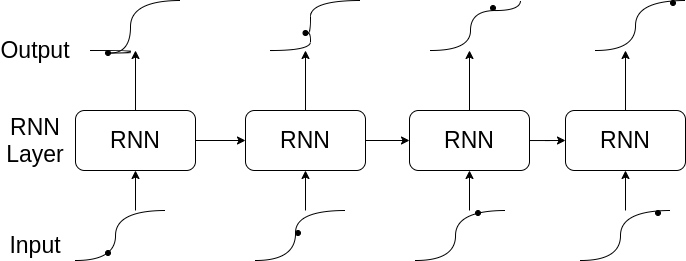
\includegraphics[scale=0.5]{RNN.png}
\end{figure}
The more rigorous definition of an RNN hidden state is as follows:
\begin{align*}
h_t = \tanh\left( W_{ih}x_t + b_{ih} + W_{hh}h_{t-1} + b_{hh}  \right)
\end{align*}
With $h_t$ being the hidden state at some time $t$ that is passed forward to the next recurrent unit at $t+1$. $W_{jj}$ is some weight matrix, $x_t$ the input vector and $b_{jj}$ some bias vector. \\

RNNs perform well on sequential data, however, in large time scales the model is likely to suffer from poor long term memory due to repeated gradients diminishing exponentially in time, the so called vanishing gradients problem. An additional contributor to the standard RNNs poor long term memory is that after each RNN cell we pass data through an activation function, which over many repeated transformations can result in loss of information in the data. 
\subsection{LSTM}
\label{sec:LSTM}
Long short-term memory (LSTM) is an extension to the idea of an RNN in that sequential data can be predicted by passing the hidden state of LSTM cells forward in time, however, a more sophisticated design of each unit in an attempt to mitigate information loss due to repeated data transformations and the vanishing gradients problem. The overall architecture of the LSTM cell is displayed bellow and in the following sub sections I will break down what each piece of the cell does and why it is included. 
\begin{figure}[H]
\caption{LSTM cell \cite{LSTM}}
\label{fig:RNN}
\includegraphics[scale=0.4]{LSTM_cell.png}
\end{figure}
The above figure is complex, however, we can decompose the operations into four distinct functional components ("Gates") namely: Learn, forget, remember, and use gates. Each of these four gates has a specific intended function, however, it is pertinent to note that with most statistical models there is little rigorous reasoning to their structure. By combining the following gates (or adding new ones) in novel ways one can form their own cell with desired properties. Another cell commonly referred to in the literature is the Gated Recurrent Unit (GRU) which has a lower computational cost than the LSTM as it only uses two gates, namely the update and reset gates.\\
Note: The cell state is sometimes referred to as the long term memory and the hidden state the short term memory.
\subsubsection{The Learn Gate (Input gate)} 
The Learn gate determines which information from the hidden state and input should enter the cell state. This is accomplished by passing the previous hidden state $h_{t-1}$ and input $x_t$ through a sigmoid (producing $i_t$) and $\tanh$ activation ($g_t$) functions and combining the results in point wise multiplication.
\subsubsection{The Forget Gate} 
The forget gate $f_t$ is included to determine which information can be ignored or emphasised. The forget gate takes in some input $x_t$ and some previous hidden state $h_{t-1}$ which are passed through a sigmoid activation function. The result of the sigmoid function is between 0 and 1 with 0 implying the data is irrelevant and a 1 indicating the data is highly valuable. The output of the forget gate is then used in the cell state operation to find $c_t$.
\subsubsection{The Remember Gate (Cell State)} 
The remember gate is, in essence a combination of the previous cell state $c_{t-1}$ with the information produced by the forget gate (using point wise multiplication) and then the input gate $g_t i_t$ using point wise addition to produce a new cell state $c_t$. This scheme is an attempt to calculate the most valuable new cell state.
\subsubsection{The Use Gate (The output gate) } 
The use gate is used to produce the new hidden state $h_t$ using the most relevant information from the previous hidden state $h_{t-1}$, input $x_t$ and cell state $c_t$. First we process the previous hidden state and input by passing them through a sigmoid activation function, the result being some $o_t$. Then we can calculate the new hidden state $h_t$ by point wise multiplying $o_t$ and the result when passing the cell state through a $\tanh$ activation function.

\subsubsection{Rigorous representation of LSTM operations} 

With the macro definition of the LSTM cell we can print the rigorous mathematical definition which is as follows \cite{LSTM}\cite{sak_senior_beaufays_2014}:
\begin{align*}
&i_t = \sigma\left(W_{ii}x_t + b_{ii} + W_{hi}h_{t-1} + b_{hi} \right) \\
&f_t = \sigma\left(W_{if}x_t + b_{if} + W_{hf}h_{t-1} + b_{hf} \right) \\
&g_t = \tanh\left(W_{ig}x_t + b_{ig} + W_{hg}h_{t-1} + b_{hg} \right) \\
&o_t = \sigma\left(W_{io}x_t + b_{io} + W_{ho}h_{t-1} + b_{ho} \right) \\
&c_t = f_t \odot c_{t-1} + i_t \odot g_t \\
&h_t = o_t \odot \tanh(c_t)
\end{align*}
Where $\sigma$ is the sigmoid function, $\odot$ is the Hadamard product (element wise product), $c_t$ is the cell state at some time, $h_t$ is the hidden state at some time, $i_t$ is the input gate, $f_t$ is the output gate, $g_t$ the cell gate, $0_t$ is the output gate and $x_t$ is the input data at some time. $W_{jj}$ are the input weights and $b_{jj}$ is the input bias. 
\section{NoizeNet}
\label{sec:nn}
\subsection{Data and pre-processing}
The data used for training, validation and prediction is from the free music archive which includes songs labelled with many useful characteristics, particularly interesting to us is genre.  \cite{fma_dataset}
\cite{fma_challenge}
\subsubsection{Digital Music}
In this section I will briefly discuss why RNN's are a favourable model of choice for digital music generation. \\
Sound is fundamentally a time series phenomenon, being the pressure of a medium in space. When we sample sound using a microphone, we record the voltage changes in an inductor that is actuated by the changing pressure of the air. These voltage values can then be scaled by some scaling function determined by a manufacturers calibration and saved. The output file can then be viewed as many amplitude values in some complex wave traveling in time. There is some complexity with compression formats such as the mp3 standard which are taken care of by the librosa library. \cite{isoMP3}
\subsubsection{An introduction to digital sound representations}
Now that it is clear how digital audio is stored, in this section I will briefly discuss the different representations of digital audio and why we use them. \\
Firstly, following from the above section on digital music we can see the sample or wave view which is an intuitive plot showing the sample amplitude against time. These plots are useful to us for checking the quality of the data produced by our model as we can clearly see if there is any erratic non-music like data. This view, however, gives us little indication of the qualitative aspects of the music produced by a model. 
\begin{figure}[H]
\centering
\caption{Example wave view Ref. \cite{mcfee2015librosa}}
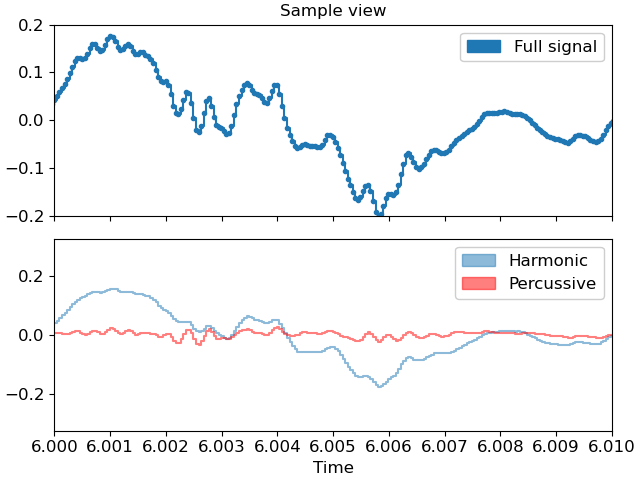
\includegraphics[scale=0.5]{librosa-display-waveshow-1_01.png}
\end{figure}
The next representation to be aware of is the envelope view which shows the amplitudes as did the sample view, however, this view makes reading off qualitative aspects of the music simple. The envelope is often used by musicians, who will often use the ASDR interpretation of each progression in the graph. \cite{vail_2013}
\begin{figure}[H]
\centering
\caption{Example Envelope view Ref. \cite{mcfee2015librosa}}
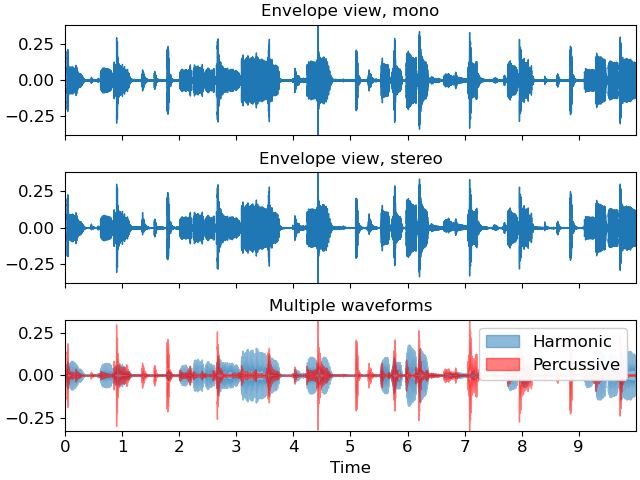
\includegraphics[scale=0.5]{librosa-display-waveshow-1_00.png}
\end{figure}
The last audio representation we will use in this paper is the spectrogram which is a heat map with frequency (logarithmic or linear) on the vertical axis, time on the horizontal axis and temperature representing volume. The spectrogram is often used in scientific audio applications as it gives us a clear plot showing the distribution of frequency and volume which we can use to describe both qualitative and quantitative aspects of the data produced by a model. 
\begin{figure}[H]
\centering
\caption{Example spectrogram Ref. \cite{mcfee2015librosa}}
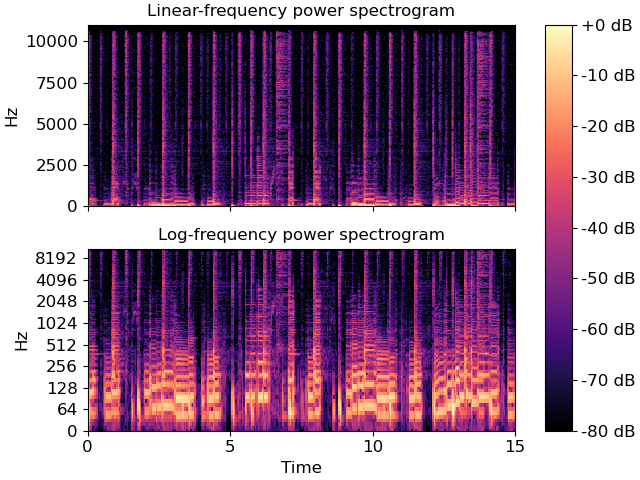
\includegraphics[scale=0.5]{librosa-display-specshow-1.png}
\end{figure}
\label{sec:data}

\subsubsection{Additional data representation}
Now that it is clear how digital music is represented and viewed we can discuss an additional representation of the data. The musical data in its current format although periodic, is highly nonlinear as decisions made by the artist are somewhat arbitrary without much underlying variable dependence. This is especially true in modern music where traditional notes, tempo and other musical norms are ignored, favoring intuitive qualitative enjoyment of a song. This philosophy to music design results in the underlying sound data being highly erratic and nonlinear which necessitates a more complex model to capture the highly nonlinear behavior. In the two figures bellow one can see the differences between a classical and a modern instrumental song.
\begin{figure}[H]
\caption{Envelope plots demonstrating classical vs instrumental music behavior}
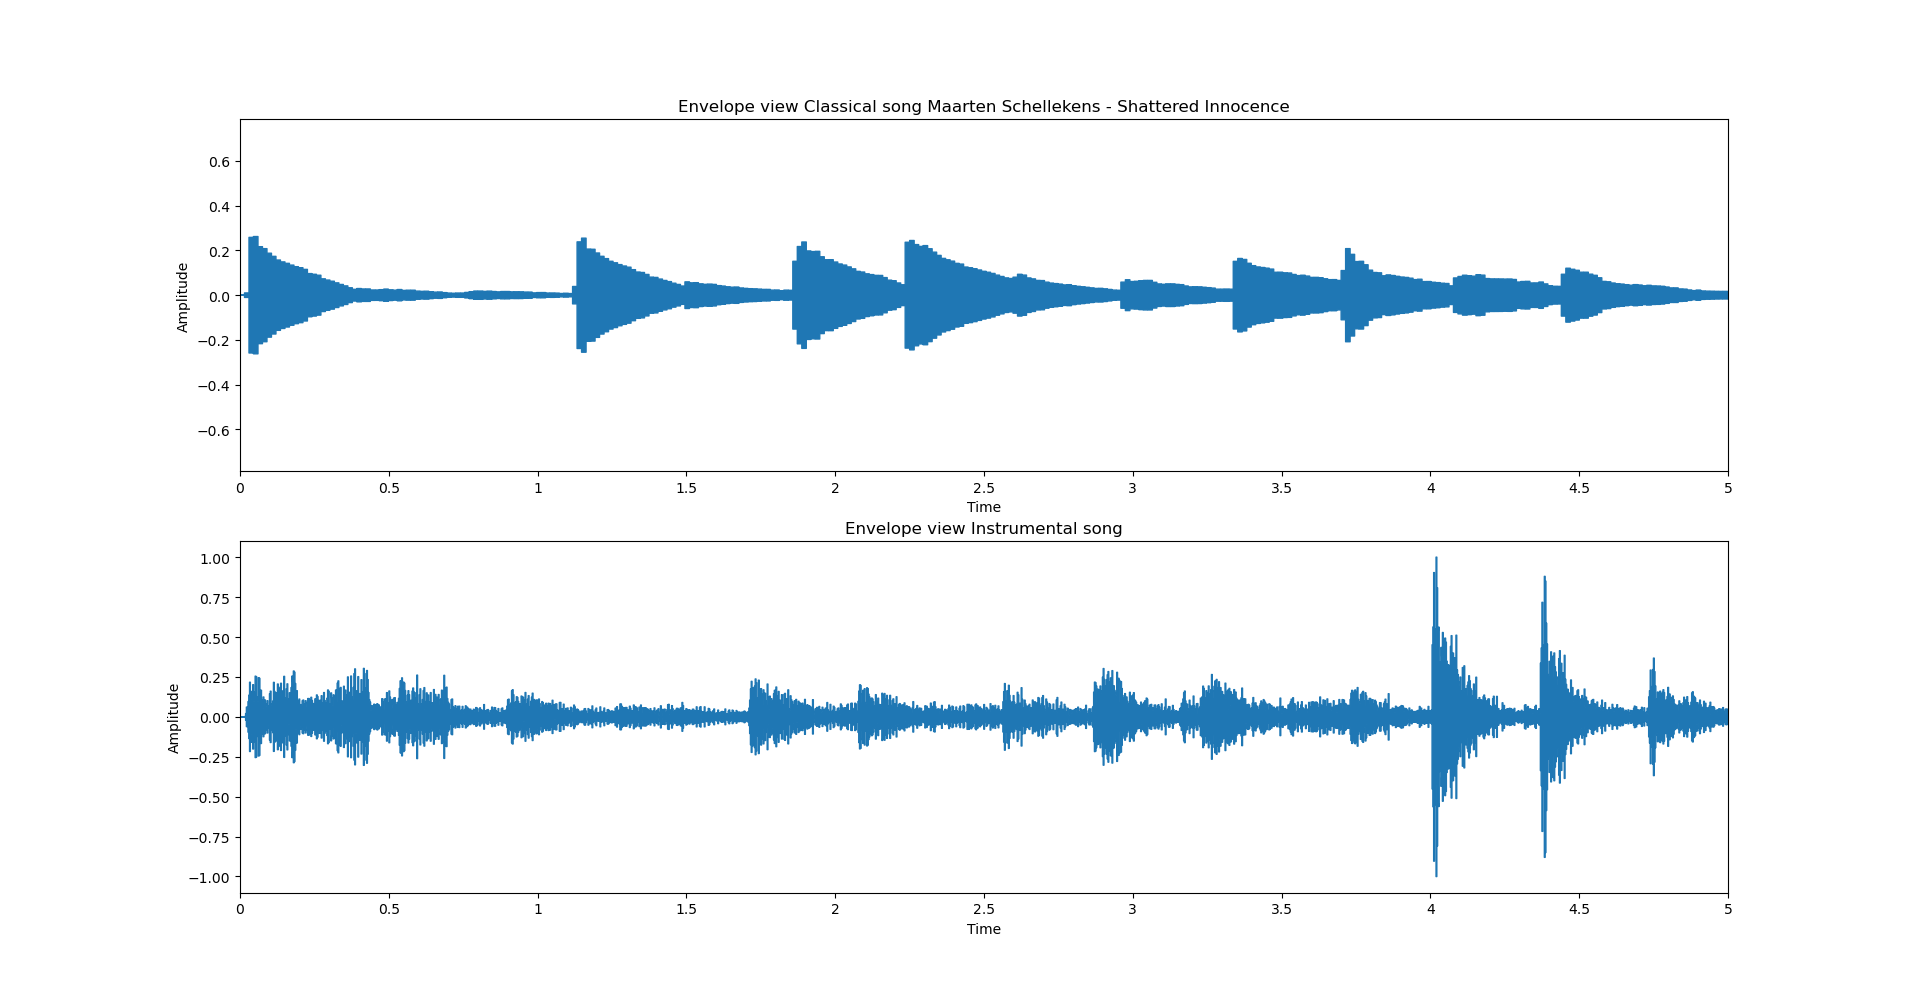
\includegraphics[scale=0.35]{Classical_vs_Instrumental.png}
\end{figure}
In order to extract more useful information from the data we can transform some input song using a discreet Fourier transform (namely the fast Fourier transform scheme (FFT)). A Fourier transform of the amplitude domain data results in frequency domain data. This new representation should better yield temporal frequency information such as chords or notes to the model and thus require lesser training time or model complexity. Bellow we can see a modern instrumental song in amplitude and frequency domains. 
\begin{figure}[H]
\caption{Envelope plots demonstrating classical vs Instrumental music behavior via FFT}
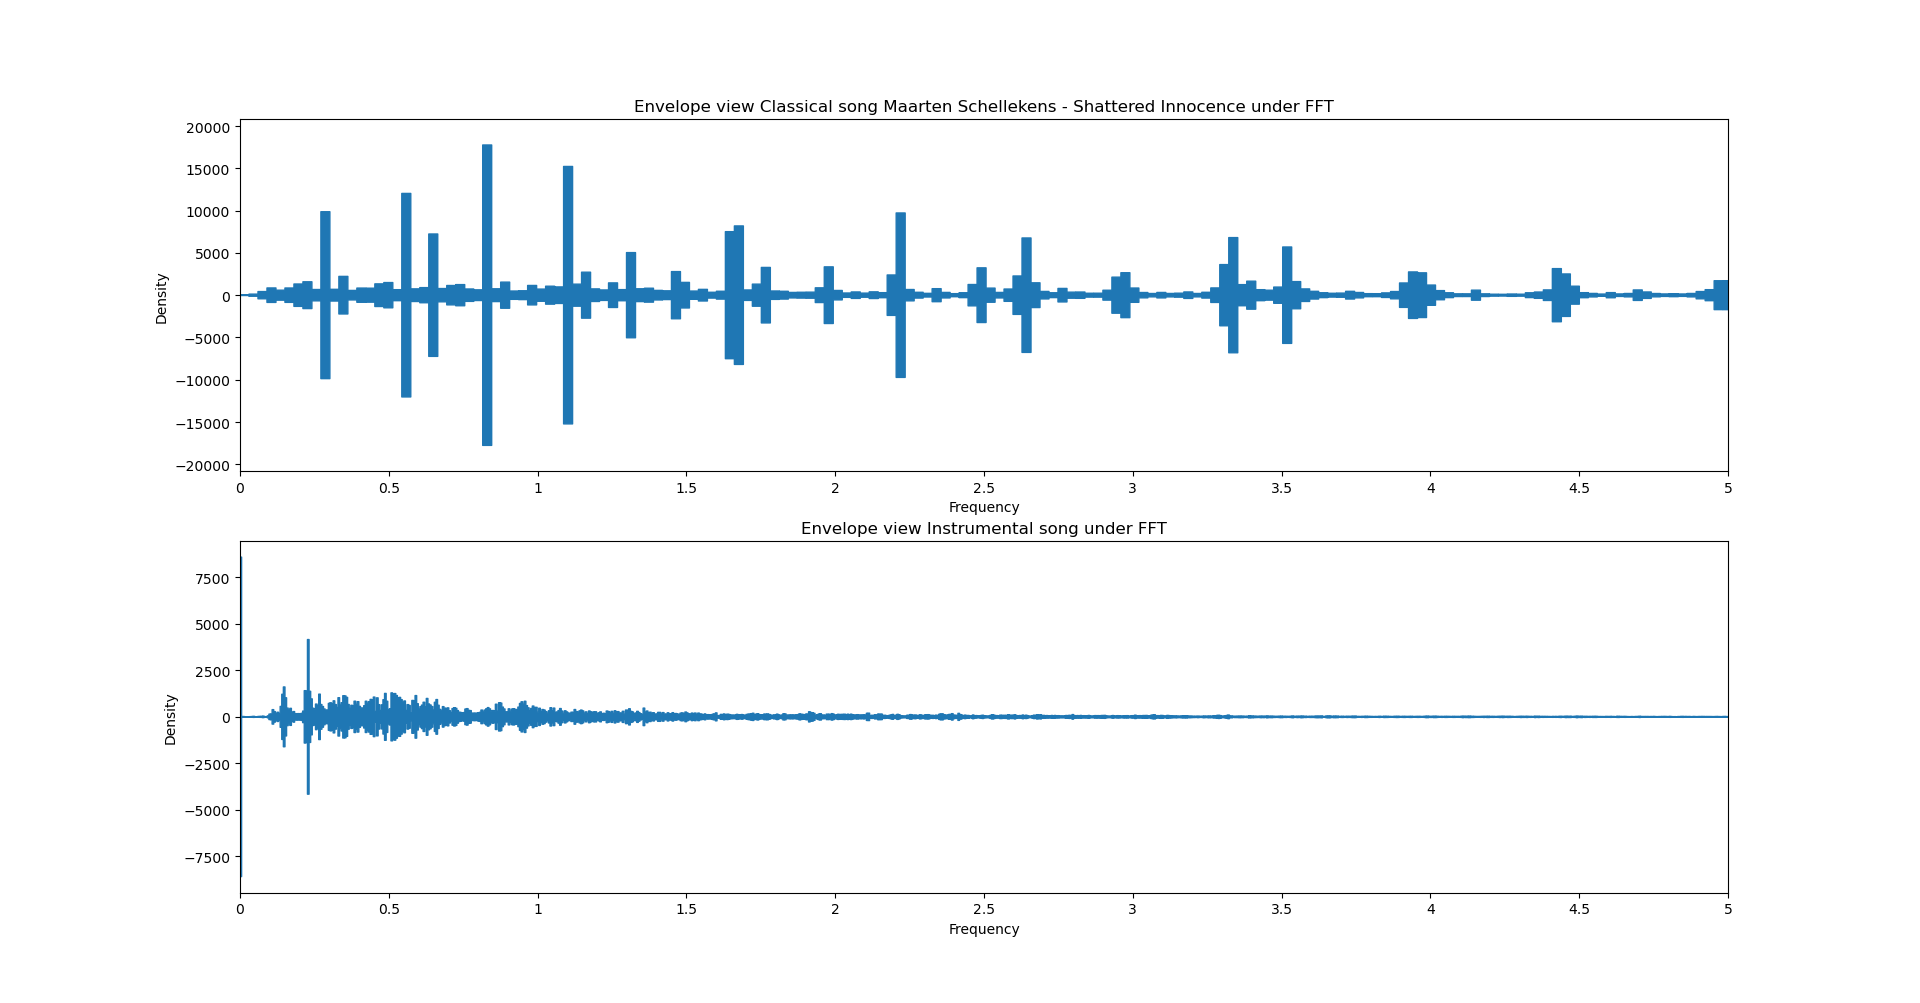
\includegraphics[scale=0.35]{Classical_vs_InstrumentalFFT.png}
\end{figure}
\subsubsection{Data used for generation seed}
In order to generate novel music we need to give the model some initial data to being prediction, referred to as the seed. In this work we will be using three different seeds namely: An unseen instrumental song, random noise and perlin noise.
\begin{enumerate}
\item The instrumental song used as a seed is completely unseen by the model. That is to say the seed is not in the training data. We expect this seed to produce the highest quality results as it is the most similar to the data used in training.
\item The random noise is generated from numpy's pseudo random normal number generator and qualitatively sounds like static noise \cite{harris2020array}. The reason for the inclusion of this seed is to experiment with how well the model retains an understanding of music when given a completely random input.
\item The perlin noise is included as an interesting sub set of the random seed as perlin noise contains qualitatively recognisable sounds which may aid the generation of novel music. How perlin noise works is beyond the scope of this paper but for the readers convenience $\mathbf{\href{https://adrianb.io/2014/08/09/perlinnoise.html}{here}}$ is an explanation.
\end{enumerate}

\pagebreak

\subsubsection{Data scaling}
Scaling the input data is an important step in the pre-processing for many reasons. Here is a list of the reasons to scale data:
\begin{enumerate}
\item Prevent neuron saturation
\item Emphasize important relations in the data
\item Smoothing input data 
\item Aiding stable convergence of gradients
\item Prevents likely hood of over-fitting
\end{enumerate}
There are many different data scaling techniques which may perform differently on different data sets. A list of the most common techniques:
\begin{enumerate}
\item Linear Scaling
\item Clipping 
\item Log Scaling
\item Z-score
\end{enumerate}
In this paper work we will use Z-scaling as data scaling includes negative values and performs well under testing. It should be noted, however, that as with most choices here the choice is heuristic based and there may be a choice that performs better under certain conditions. The implementation makes use of scikit learn's standard scaler\cite{scikit-learn}.
\subsection{Architecture of NoizeNet}
\label{sec:arch}
Due to music having natural time dependence and periodicity it is wise to develop some recurrent architecture. In this paper we will use a standard RNN as well as an LSTM. Both these models should produce similar predictive behavior with the LSTM expected to exhibit better long term memory characteristics than the standard RNN. \\
The architecture of the model will consist of several layers: the input layer which typically would include some kind of normalisation or embedding,  recurrent layers and a fully connected layer to translate the recurrent layers output to the output layer. These layers are depicted in the figure bellow:
\begin{figure}[H]
\centering
\caption{Example of NoizeNet architecture demonstrating how music prediction will work}
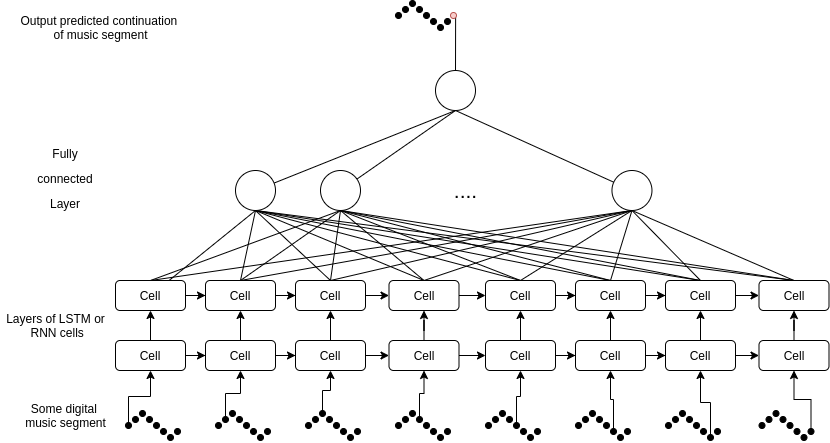
\includegraphics[scale=0.5]{NoizeNetArch.png}
\end{figure}
\subsection{Implementation}
\label{sec:impl}
The implementation for this work was completed in python with the following frameworks and libraries:
\begin{enumerate}
\item PyTorch library for Neural Networks \cite{NEURIPS2019_9015}
\item Librosa for audio I/O \cite{mcfee2015librosa} 
\item Matplot lib \cite{Hunter:2007} and Librosa display \cite{mcfee2015librosa} for graphics rendering
\item Scikit learn \cite{scikit-learn}, pandas \cite{reback2020pandas} \cite{mckinney-proc-scipy-2010}, librosa \cite{mcfee2015librosa} and numpy \cite{harris2020array} and FMA utils \cite{fma_dataset}\cite{fma_challenge} for data processing 
\end{enumerate}
Please see the code repository $\mathbf{\href{https://github.com/Liam-Watson/NoizeNet}{here}}$. Included in the repository are the figures used in this paper, an implementation of the NoizeNet model, a few saved models with varying hyperparameters that will be analysed bellow along with some output predictions and the seeds used to generate them. 

One should note that the implementation yields many hyperparameters that can be used to optimise the results produced by a model or computational performance. This is important to this investigation as audio data is very large. The sample rate used in this implementation is 22050Hz, so for a 30 second section of music we find $6.615\cdot 10^{5}$ data points. The large size of data implies, necessarily a large model and complex model, many training/prediction steps and high memory usage. Training on a very small subset of a song will not produce any music like predictions from the model as it will not have seen the macroscopic behavior music during training. \\
Due to this many hyperparameters had to be tuned for computational performance rather than model optimization. \\
The high memory requirement is also of note as one has to ensure that any unused memory is cleaned up frequently by the garbage collector. In python this is a relatively trivial procedure but is of note. 

\subsubsection{Hyper-parameters}
There are many factors that can effect a recurrent model's performance, the factors that one can control are referred to as hyper-parameters. In the table bellow I have included some of the hyperparamets that may influence both the recurrent models' ability to model musical phenomena as well as the influence on the computational cost of the parameter.

\begin{tabularx}{0.8\textwidth} { 
  | >{\raggedright\arraybackslash}X 
  | >{\centering\arraybackslash}X 
  | >{\raggedleft\arraybackslash}X | }
  \caption{Showing the hyper parameters that may influence the model performance or computational}\\
 \hline
 hyper-parameter & Influence on model & Computational cost \\
 \hline
 Hidden Layer Dimension  & A larger hidden dimension can better model nonlinear behavior. &  A larger hidden dimension increases the computational cost.  \\
\hline
 RNN/LSTM Layers  & The number of LSTM/RNN layer can better model the time series data.  &  A larger number of layers substantially increases computational cost especially for more complex cells such as an LSTM.  \\
\hline
 Loss criterion  & The influence of the loss criterion is covered in section 3.6.  & For the purposed of this paper we can assume the loss criterion's computational cost negligible. \\
\hline
 Optimizer  & An optimizer can effect the performance of a models training substantially by ensuring that an optimal set of weights are found.  &  Optimizers can very dramatically, including schemes with momentum. The more complex the optimizer the more computationally expensive. \\
\hline
 Learning rate  & A good learning rate can ensure the model finds a good local minimum  & The Learning rate doesn't directly influence computational cost, however it does effect the number of epochs one may train their model for.   \\
\hline
Gradient Clipping value & The influence of gradient clipping on the model performance is not clear and a decision on the value is heuristic based  & Gradient clipping has been theoretically proven to accelerate training thus decreasing the number of epochs needed during training. \cite{zhang_he_sra_jadbabaie_2020}\\
\hline
\end{tabularx}
\subsection{A note on numerical stability of the model}
During the implementation of NoizeNet there was significant numerical instability which is exhibited as NaN gradients, loss and prediction. Once numerical instability occurs there is no way to recover the model. Numerical instability is not well covered in scientific literature with only a few solutions being proposed. Numerical instability can be caused by many factors such as poor input data or choice of hyper parameters. In the literature common instabilities referred to are exploding gradients and vanishing gradients. \\
The solution to the numerical instabilities in this work were implementing a gradient clipping scheme which prevents exploding gradients by providing an upper bound for gradient values. An additional parameter effecting the stability of the model was the learning rate, which should be sufficiently small to ensure stability. There is no rigorous means to determine a suitable value for these two stability affecting variables and so they should be determined experimentally. 
\begin{figure}[H]
\caption{Showing how gradient clipping prevents exploding gradients for some chosen clip value C \cite{stanford}. }
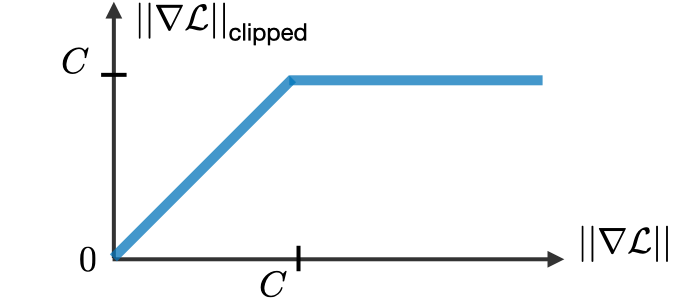
\includegraphics[scale=0.35]{gradient_clipping.png}
\end{figure}
Note that in the figure above the cost function is represented as $\pazocal{L}$.

\subsubsection{A note on batching}
An important consequence of the volume of data is the strategy for how the model will ingest it. 
There are two places where a model ingests data, namely, during training and prediction. Prediction is fairly simple, we feed the model a sufficiently large amount of data as a seed and its predicted output will then be recursively re ingested, replacing the seed.\\
However training is more complex as there are two philosophies for ingesting data, in batches or one shot. I will briefly cover why in this paper using one shot input is necessary. The general idea is that batches would be on the order of $10^4$ or less data points with a sample rate of $22050 Hz$ this equates to around a second and is considerably larger than a common batch size. Generally, music has few recognisable patterns on such time scales which is evident in the figure bellow. Due to this training must take place on larger time scales, to better recognise long term periodicity and pattern in the music. That is to say, local data patterns are unimportant to us, we only care about global, macroscopic behavior.\\
An additional factor to consider is that when batching input data is how to divide the batches. If a batch were chosen of arbitrary length, musical notes would be split in half between batches, causing the model to learn behavior that in not representative in music. 


We can see this behavior in an LSTM example that is heavily trained on batch data. The predicted output file with the first second of a song as its input seed is, in essence just noise as in a local view. The model is trained on what is essentially noise and so any prediction would resemble a similar pattern. In the figure bellow we can see clearly in the spectrogram and Envelope that there is no discernible pattern. In the Sample view we can see that samples are very erratic and show no progression over time to some frequency. 
\begin{figure}[H]
\caption{Various views showing the predicted music by an LSTM with batched training data. }
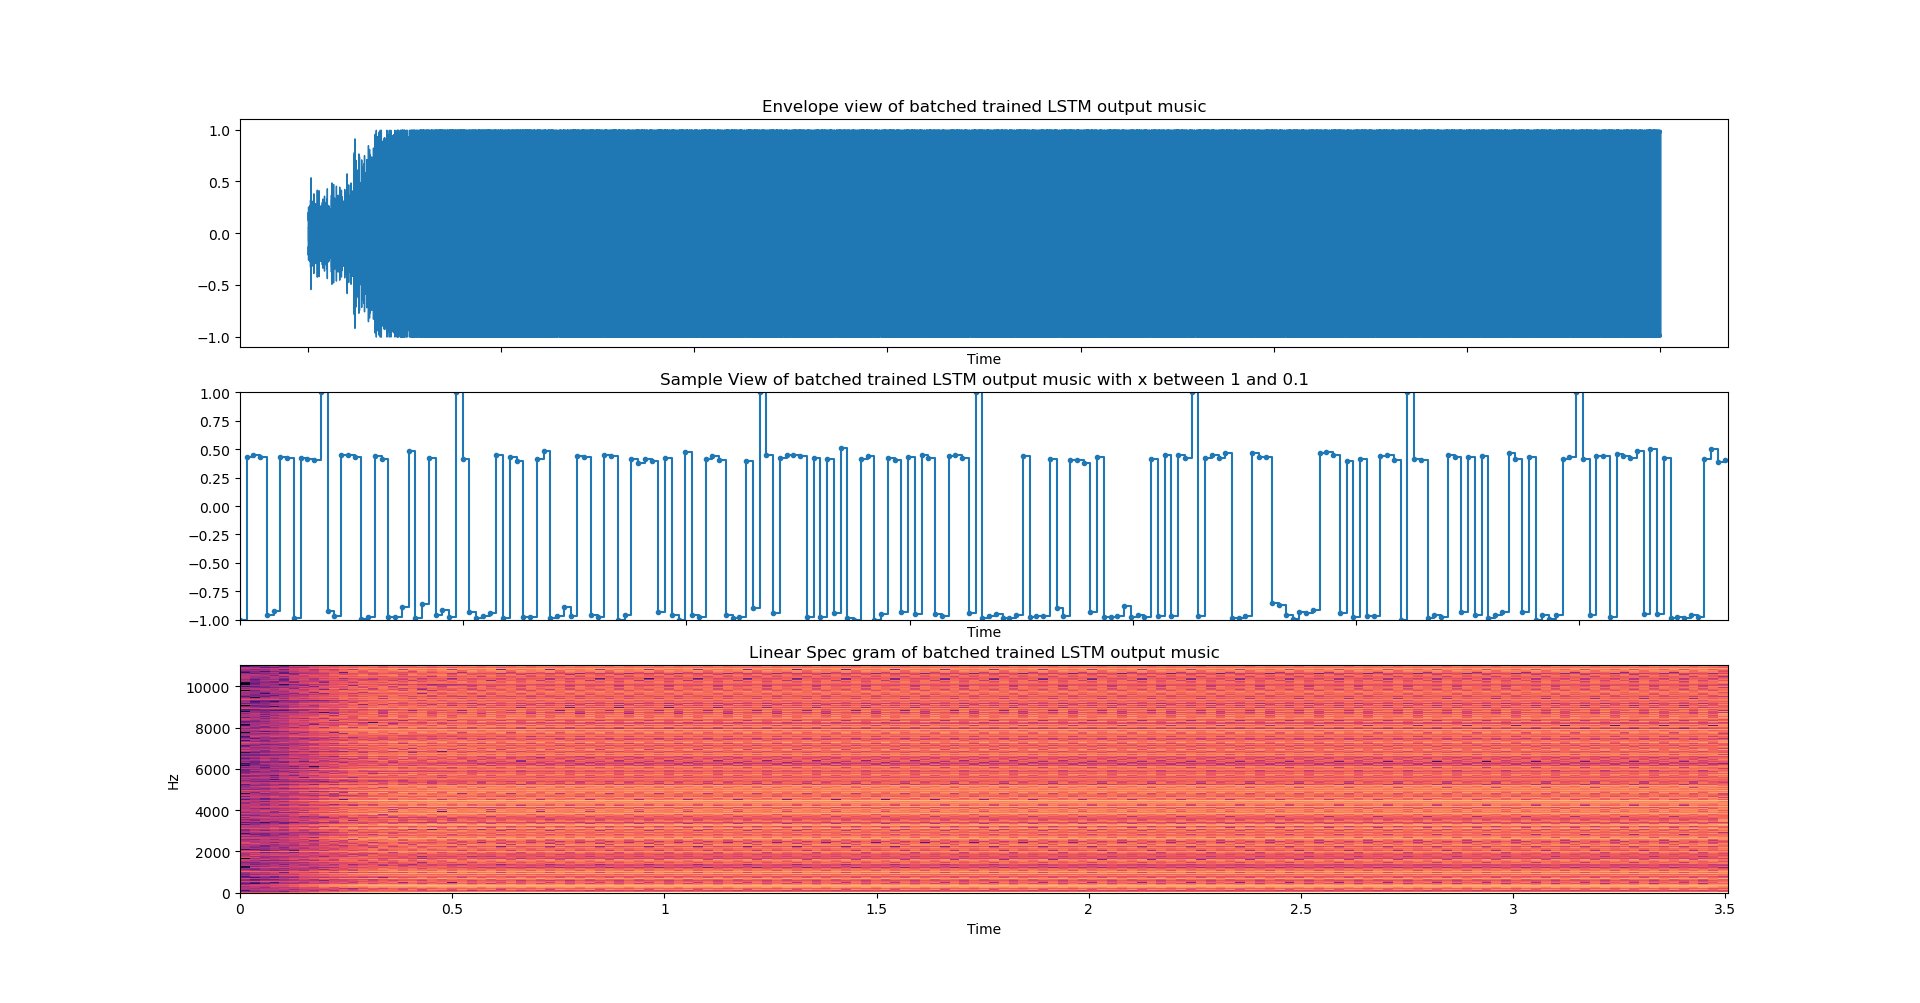
\includegraphics[scale=0.35]{batch_training.png}
\end{figure}
Due to this all training was completed in one batch in order to capture the global behavior of the song. However this strategy is more computationally intensive as each epoch one must proceed through all data points in the large input data sequence. 
\subsection{Results}
\label{sec:results}
In this section we will review various outputs of the RNN and LSTM model with various sets of hyperparameters as well analyse the qualitative and quantitative behavior of the model output. Additionally we will discuss how the results were obtained, what they may imply for the model and indeed for music generation as a whole. 

\subsubsection{Training and validation}
In this section we will discuss the results of training the RNN and LSTM by investigating loss progression as well as how well the model training generalises to unseen data via validation.

If we keep track of the loss at each epoch of training across several different songs while training we can produce a graph of the loss progression. For successful training we expect two characteristics in this graph.
\begin{enumerate}
\item We expect to see the loss decrease consistently over each epoch, indicating that the model is learning effectively from the input data.
\item We expect to see a rise in loss for each new song in the training data set. However if the model is learning more general information about the music we expect each successive song's increase in loss to decrease. It should be noted that this property may not be general as songs vary greatly in their similarity.
\end{enumerate}
\begin{figure}[H]
\caption{Plot of loss over 100 epochs of LSTM training on a single input song}
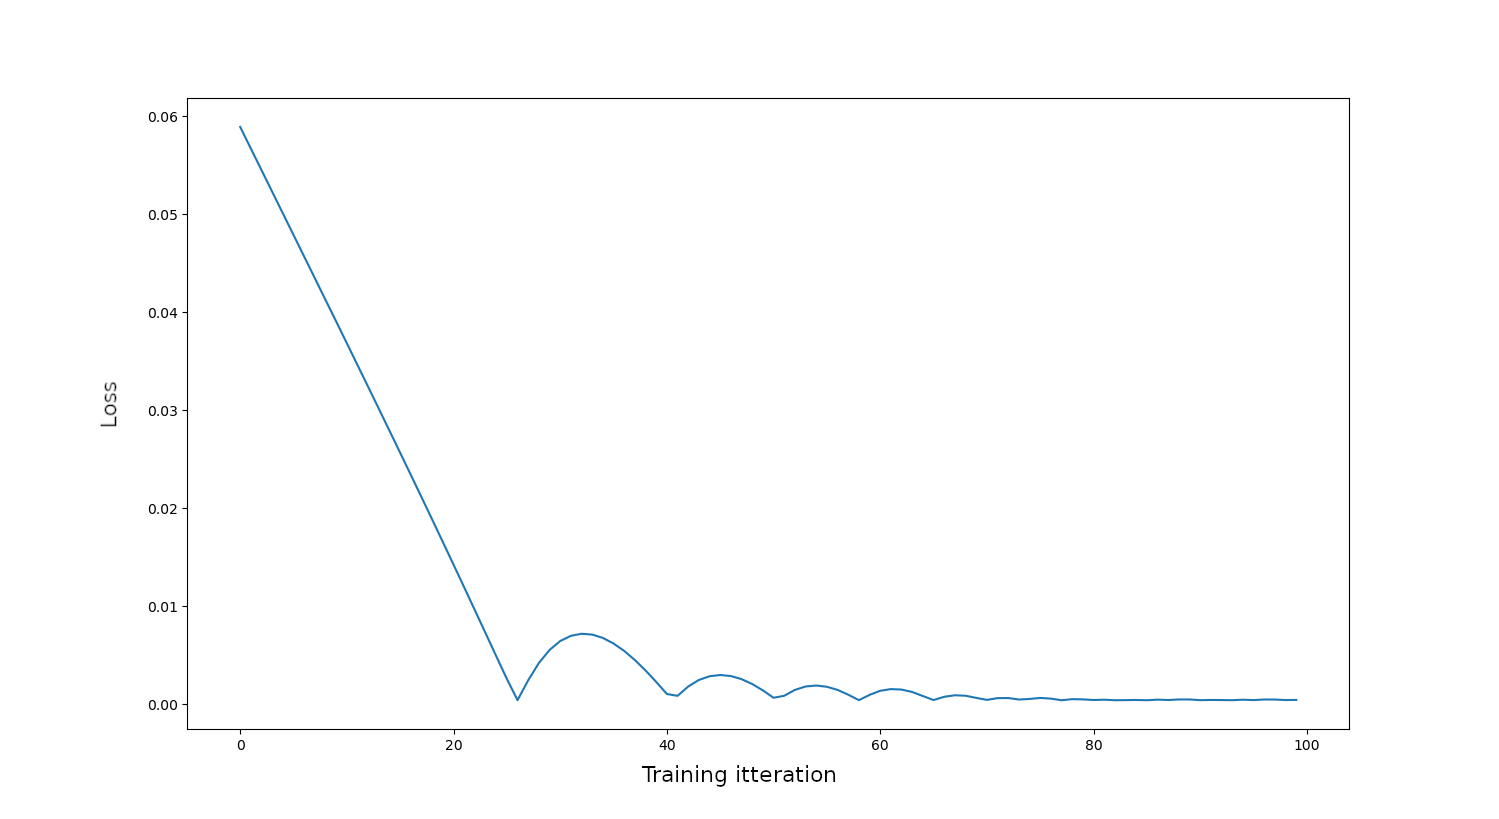
\includegraphics[scale=0.35]{loss_plot_100itr.png}
\end{figure}
Note that the loss does indeed decrease over time, however, there are two things to note. Firstly the loss has "humps" which are likely due to the optimizer attempting to find a better minimum. Secondly over time the loss settles so a near constant value, which could mean that the model is very accurate, over fitted or some other issue. If we attempt to generate a song using this model we can confirm that, indeed there is a problem with the model. This can be seen in the figure bellow where the prediction is some constant value. 
\begin{figure}[H]
\caption{Prediction of 1000 amplitude samples with a classical song as the seed}
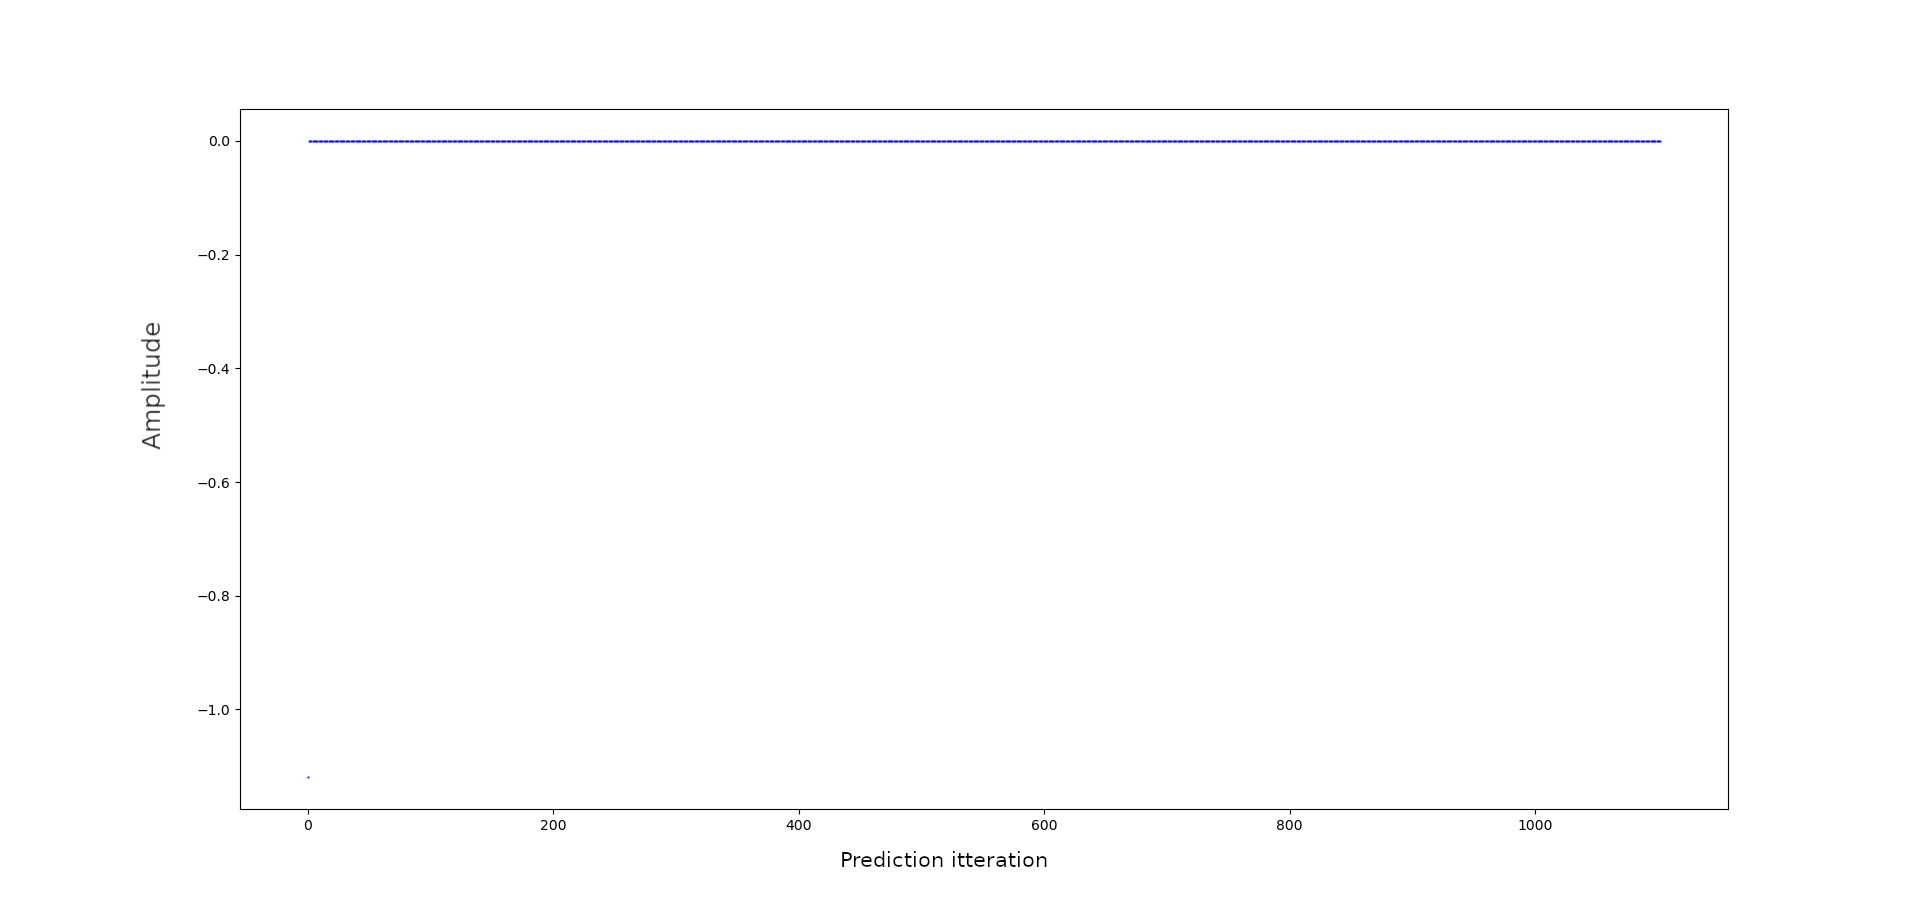
\includegraphics[scale=0.35]{overfit_1.png}
\end{figure}
Over fitting as a problem that effects most machine learning models. There are many proposed schemes to combat over fitting, a common one that we will use in this work is dropout. Dropout randomly selects arbitrary values to completely drop. In the context of RNN's we introduce a Dropout layer on the outputs of each RNN layer and randomly select values to drop. After including a dropout scheme we can see in the figure bellow that the model no longer exhibits this over fitting behavior during training. It should be noted, however, that the model does still produce a constant output prediction but it takes many more predictions to fix on a constant.
\begin{figure}[H]
\caption{Plot of loss over 100 epochs of LSTM training on a single input song}
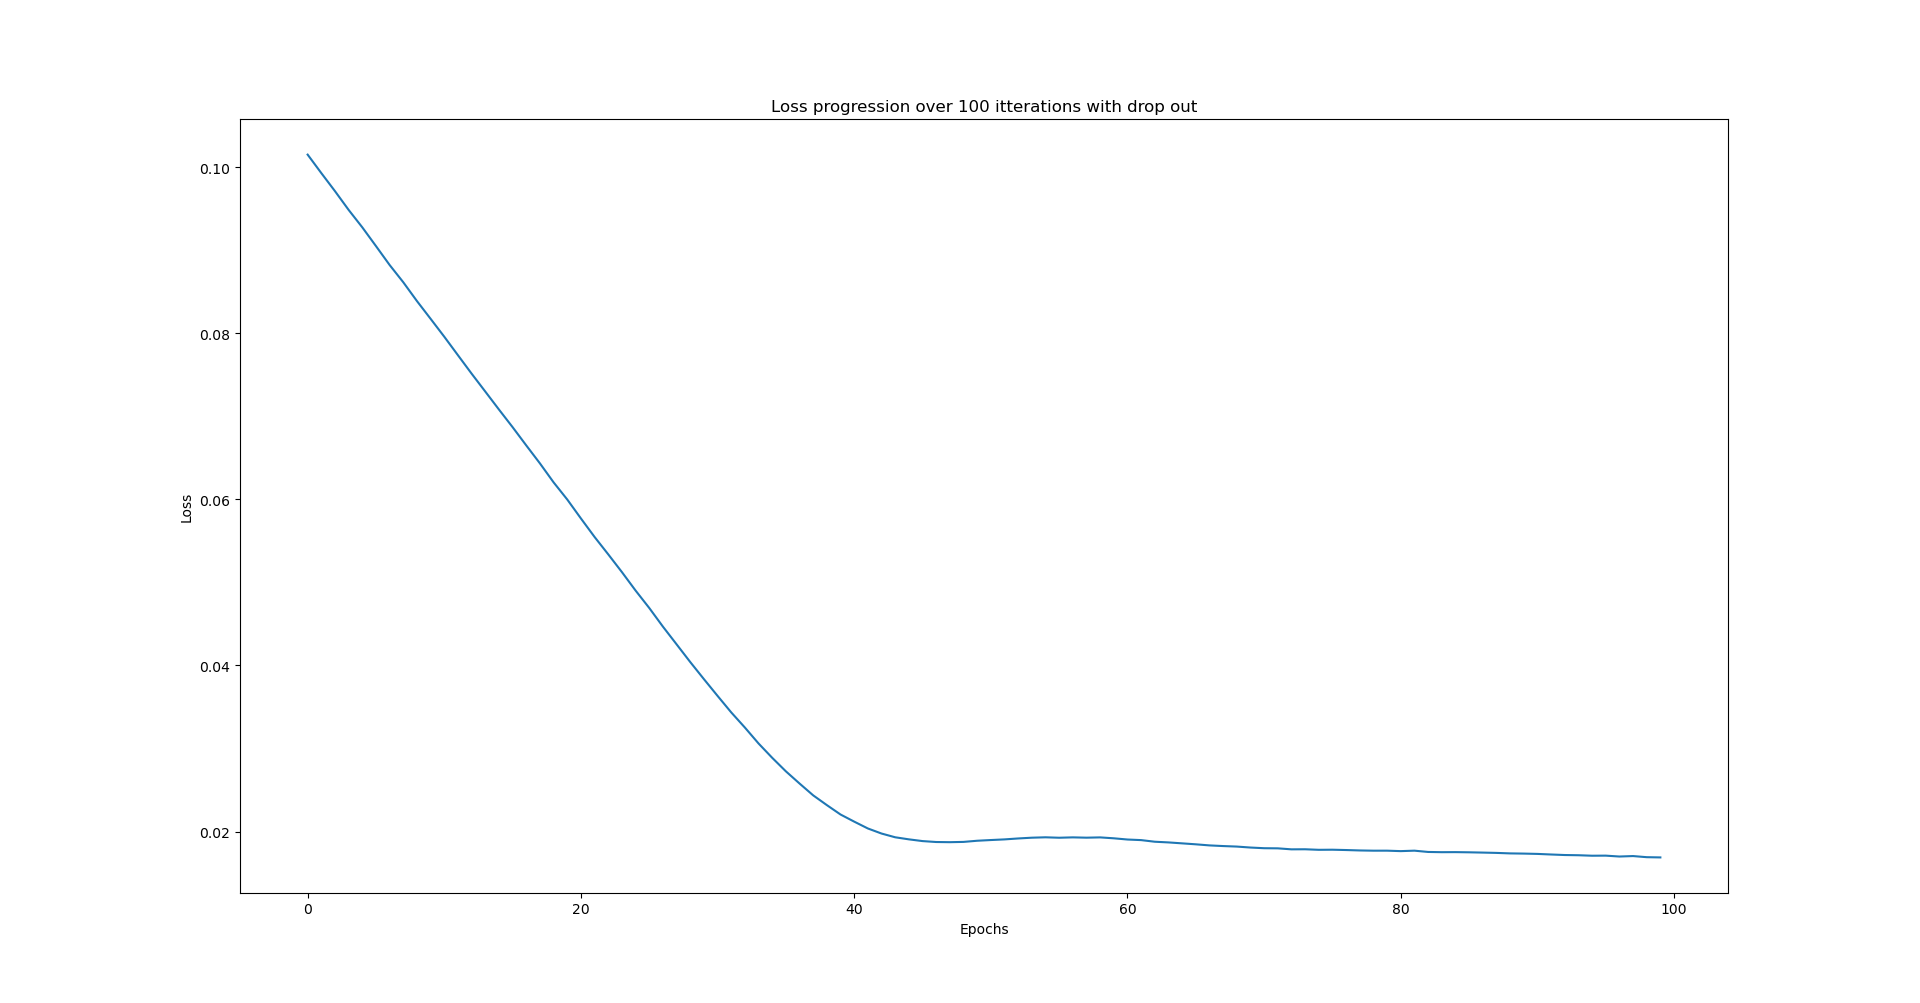
\includegraphics[scale=0.35]{loss_dropout_100itr.png}
\end{figure}
We can now verify that the model is learning generalised knowledge. First let us plot the loss progression for training over multiple songs.
\begin{figure}[H]
\caption{Plot of loss over 100 epochs with 10 songs of 10 epochs each for LSTM}
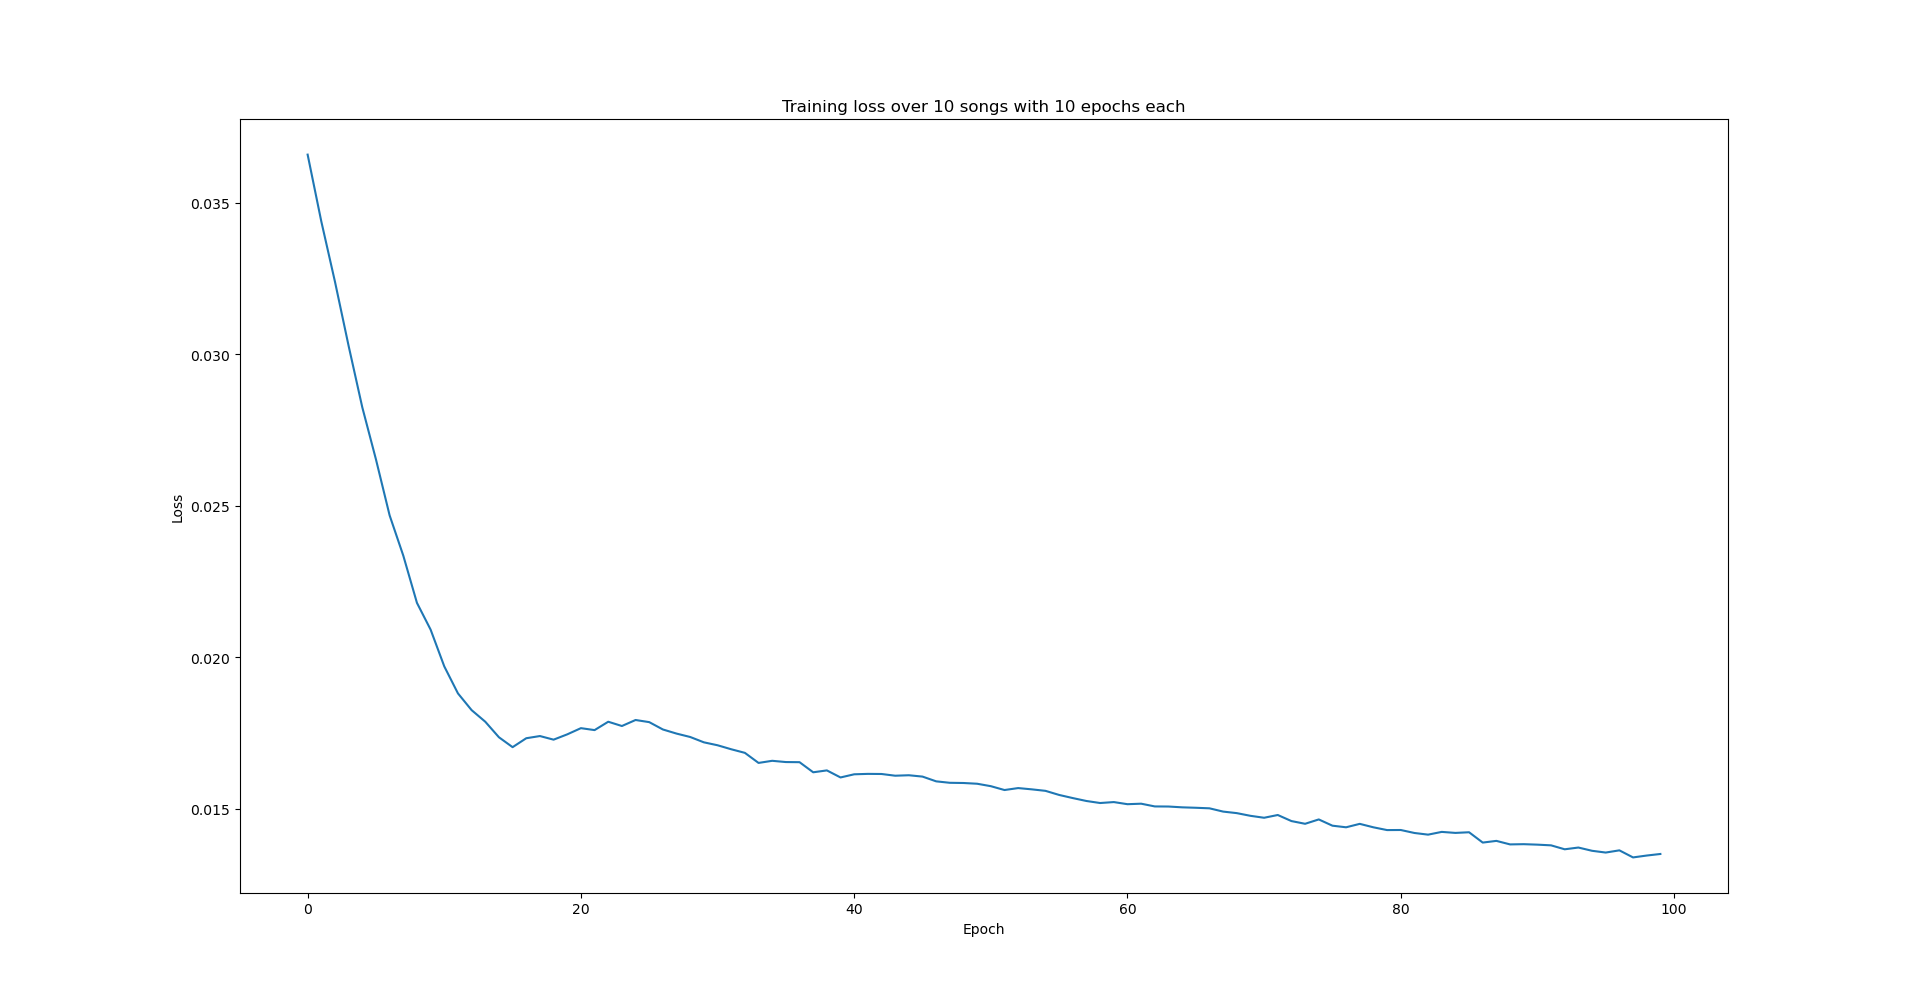
\includegraphics[scale=0.35]{loss_plot_10songs.png}
\end{figure}
After we have confirmed that the loss is decreasing as expected we need to ensure that the training is generalising to unseen data and confirm that we are not over fitting the model. To check both of these we can use a validation step during training, where periodically we give the model some unseen data as input and check the error of the prediction to the unseen data. Bellow we can see a figure showing that as the loss decreases so does the validation loss. If the model was over fit the validation loss should increase as training continues.
\begin{figure}[H]
\centering
\caption{Plot of loss over 20000 epochs with 10 songs of 10 epochs each for with validation every 100 epochs LSTM}
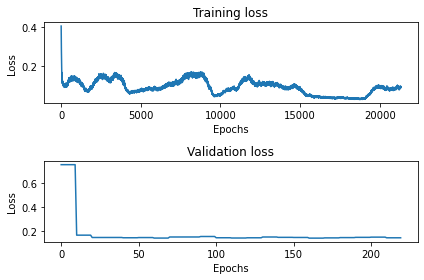
\includegraphics[scale=0.7]{validation.png}
\end{figure}
\subsubsection{Initial investigation}
Before we begin to ask our model to generate completely new music it is insightful to see if the network can reproduce music. If we train the model on raw music samples and proceed to feed it music it has not been trained on as input we find the following output.
\begin{figure}[H]
\caption{Showing the reproduction of an unseen song by LSTM}
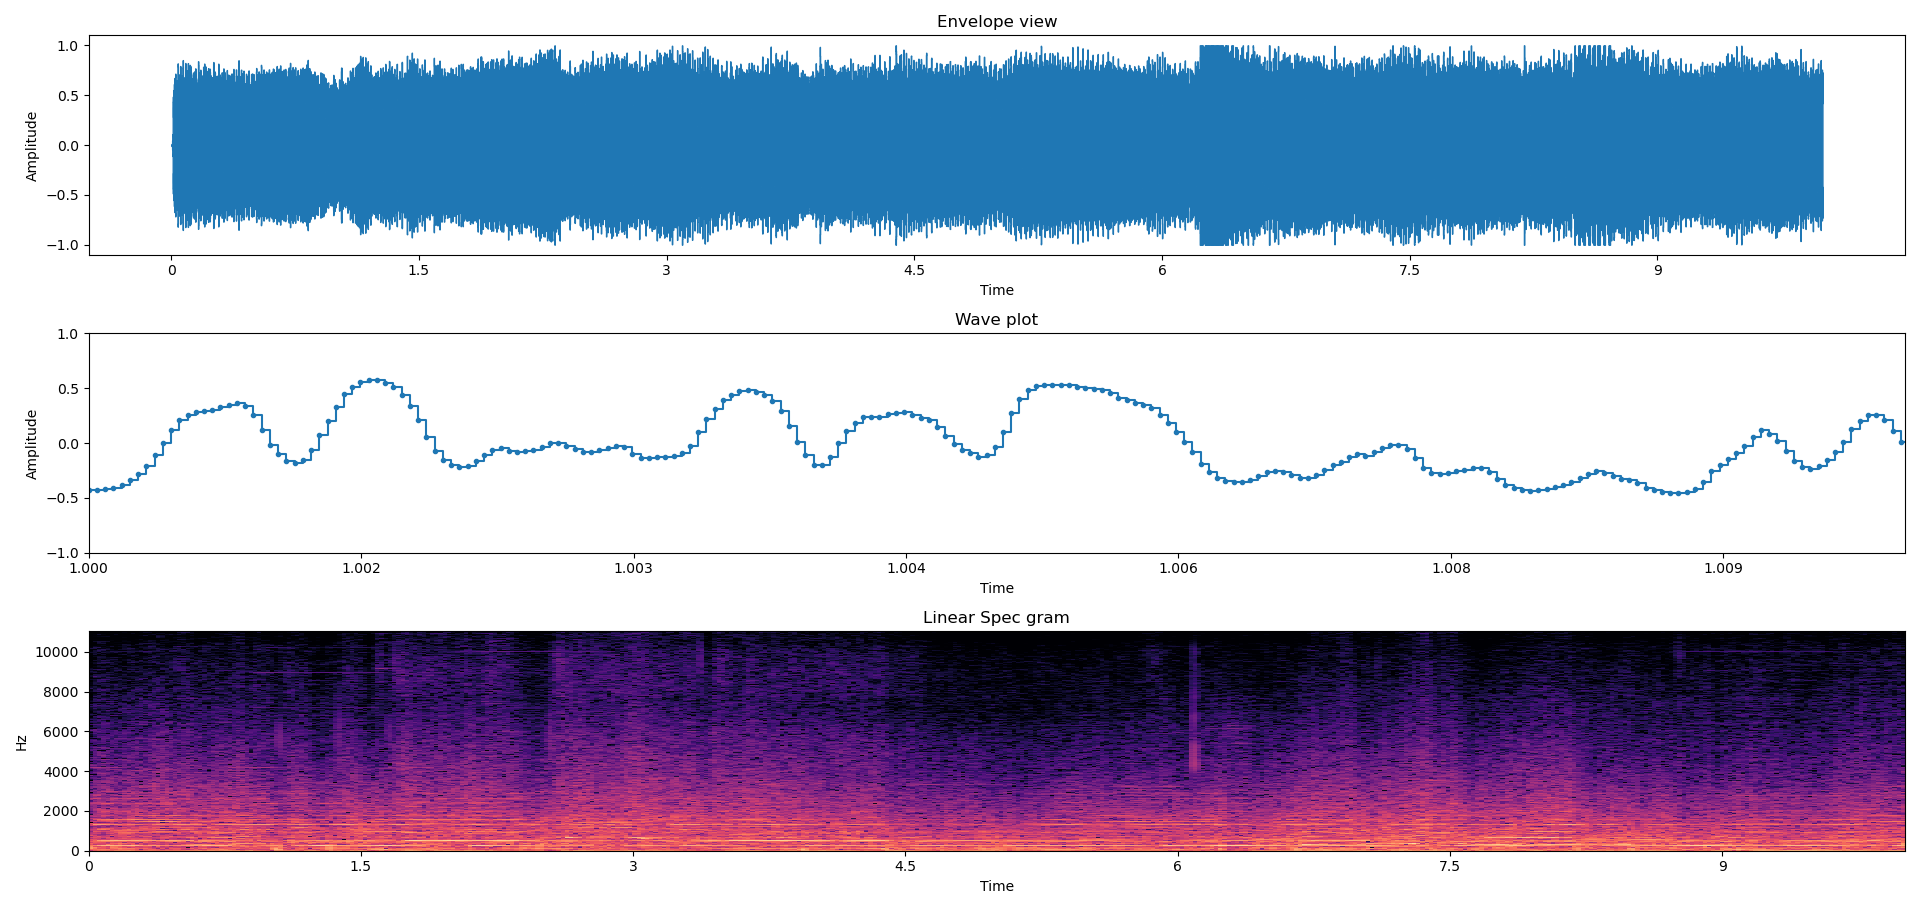
\includegraphics[scale=0.35]{reproduce1.png}
\end{figure}
We can see in the wave plot that the output is relatively smooth on small time scales with few erratic jumps. However there is still some noise in the output music which can be seen by the ill defined envelope and spectrogram. 
\begin{figure}[H]
\caption{Showing the reproduction seed of an unseen song}
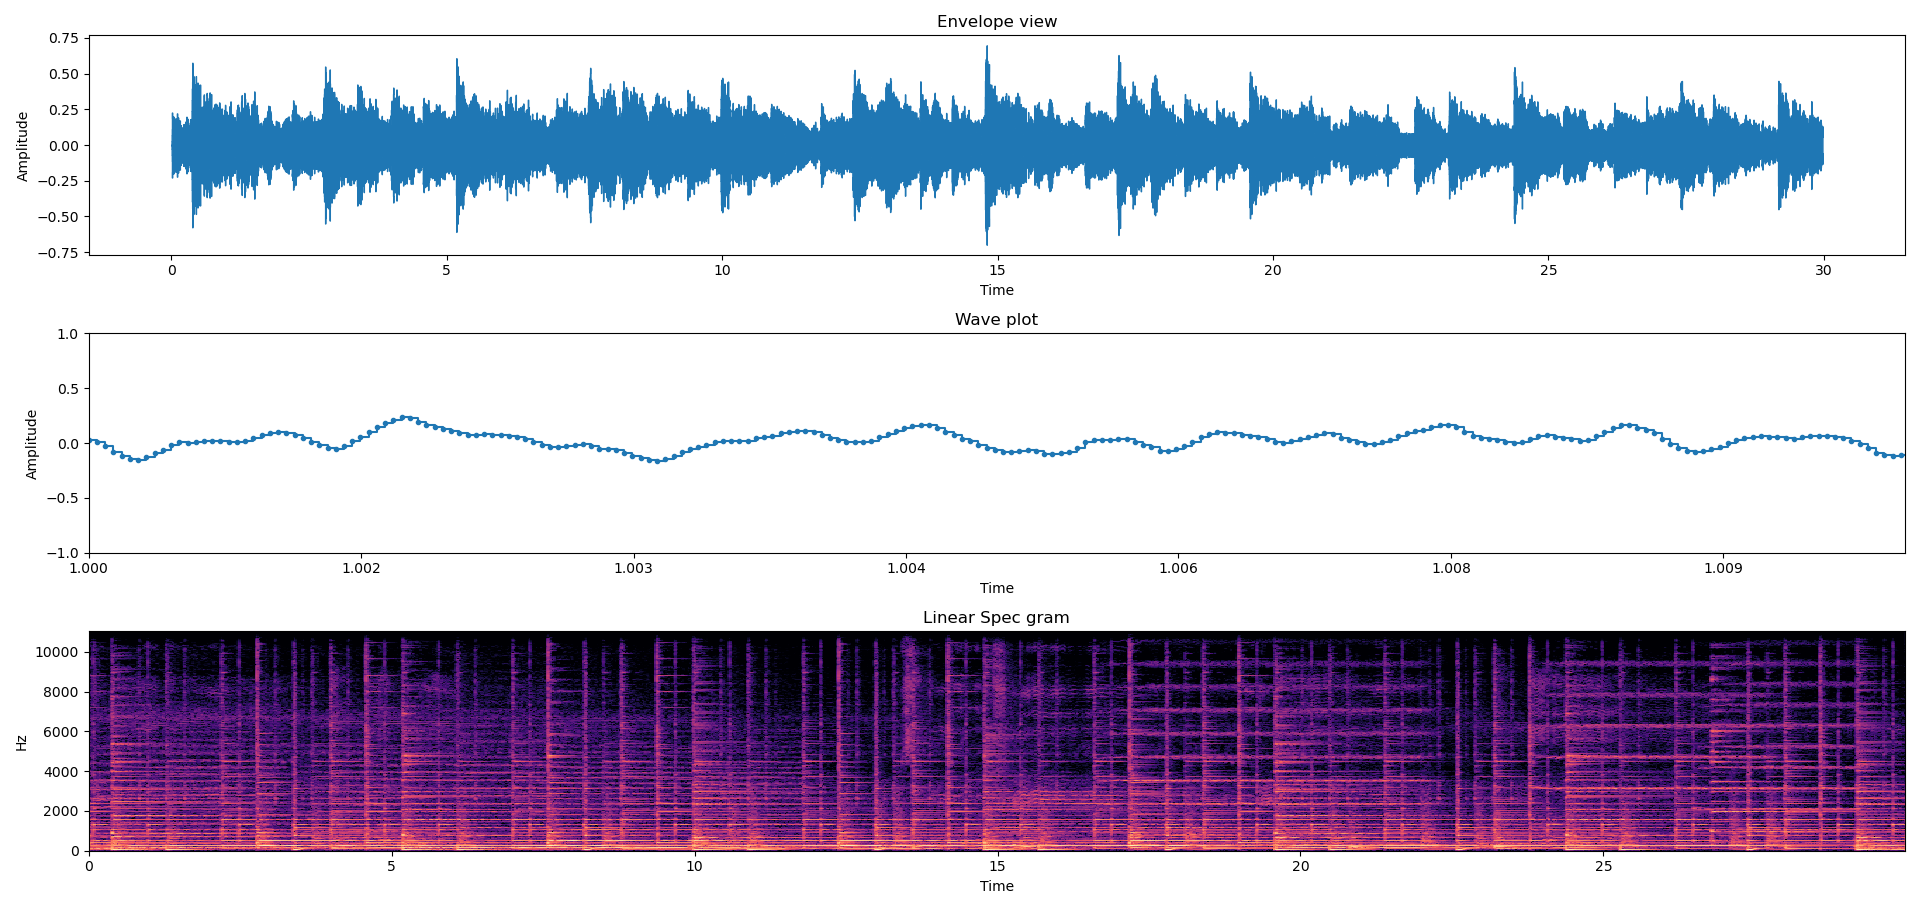
\includegraphics[scale=0.35]{reproductionSeed.png}
\end{figure}
It should be noted that although the reproduction is noisy, to the ear the music is definitely recognisable and qualitatively not unpleasant. 
\subsubsection{RNN and LSTM comparison}
Here we will compare the performance of an RNN and LSTM model with the same hyperparameters where applicable. 
For a reproduction the RNN performs slightly worse than the LSTM with the same hyperparameters. The envelope and spectrogram in the figure bellow shows that the RNN reproduction contains more noise than the LSTM. Additionally, the wave plot shows that the RNN produces more erratic output that leads to a qualitatively poor listening experience. It should be noted, however, that the reproduction is still recognisable. 
\begin{figure}[H]
\caption{Showing the reproduction of an unseen song by RNN}
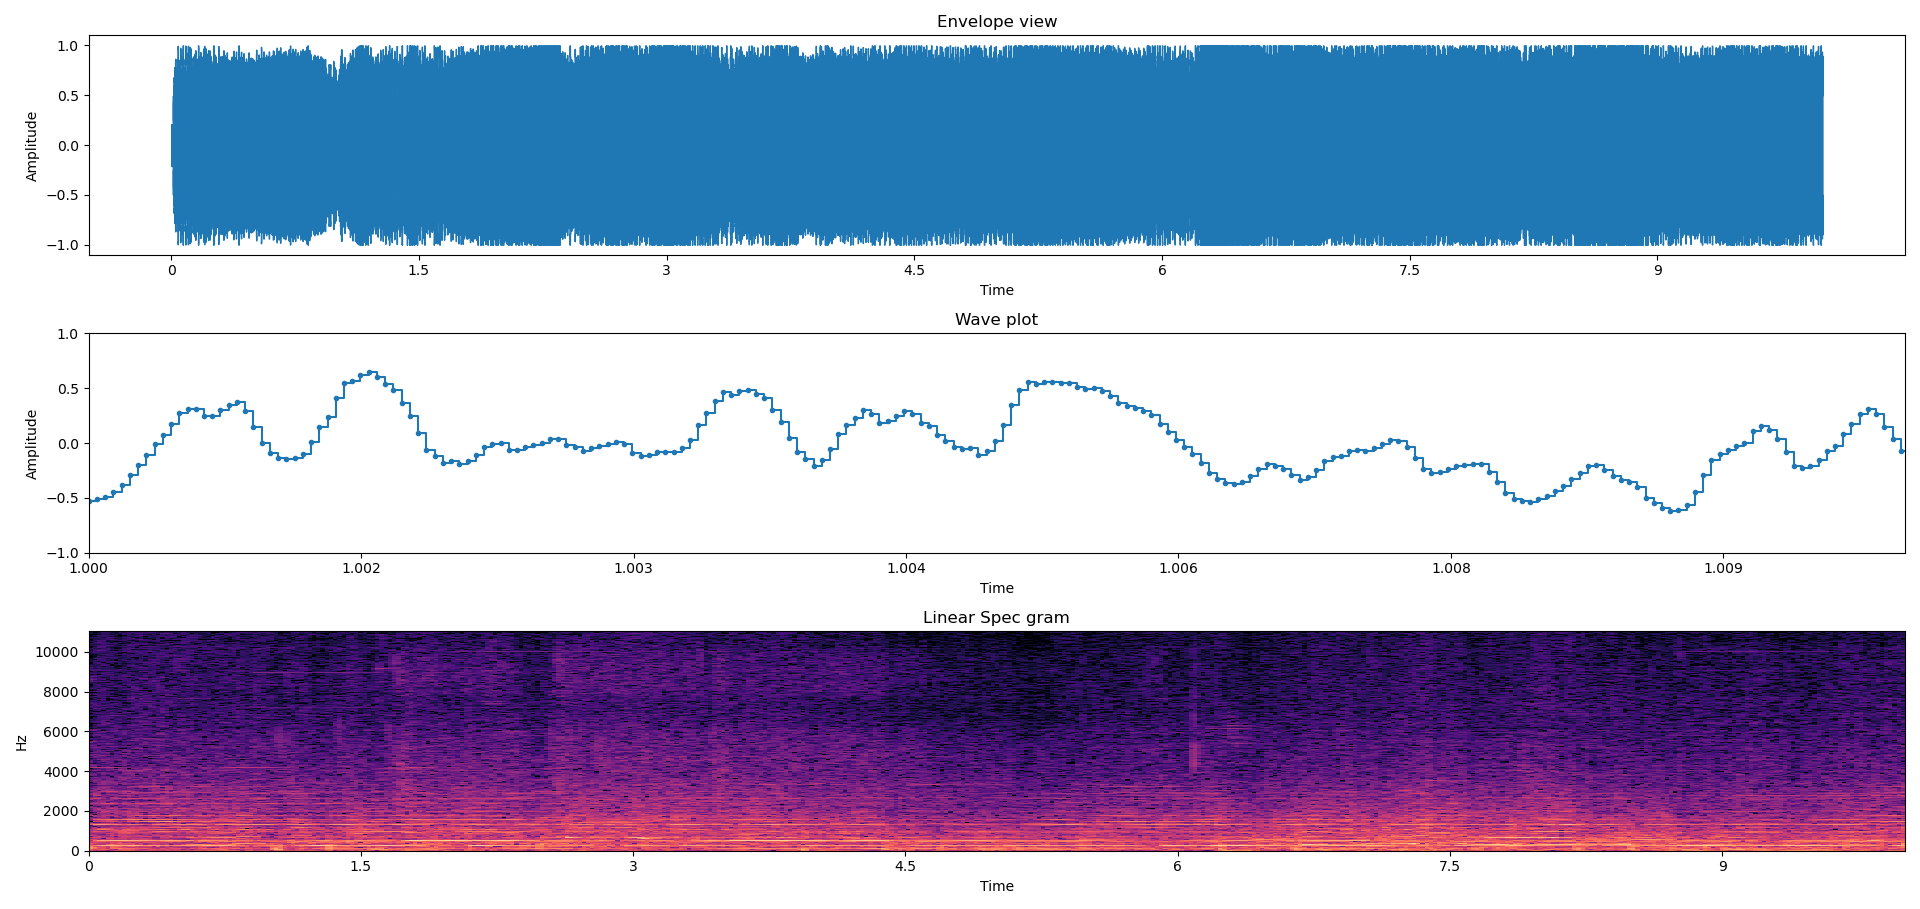
\includegraphics[scale=0.35]{RNN_Reproduction.png}
\end{figure}
The parameters are listed in the table bellow\\
\begin{tabularx}{0.8\textwidth} { 
  | >{\raggedright\arraybackslash}X 
  | >{\centering\arraybackslash}X 
  | >{\raggedleft\arraybackslash}X | }
 \hline
 Hyper-parameter & Value\\
 \hline
 Hidden Layer Dimension  & 50   \\
\hline
 RNN/LSTM Layers  & 2 \\
\hline
 Loss criterion  & MSE Loss  \\
\hline
 Optimizer  & Adam Optimizer  \\
\hline
 Learning rate  & 0.0001  \\
\hline
 Genre  & Instrumental \\
\hline
 Number of songs to train on  & 5  \\
\hline
 Duration of song to train on on  & 15s \\
\hline
Gradient Clipping value & 1 \\
\hline
Dropout probability & 0.5 \\
\hline
\end{tabularx}
After approximately 5 iterations of prediction both the RNN and LSTM converge to a single output value. After researching this problem thoroughly there appears to be no formal works discussing the topic, however, there has been some informal discussion which often leads to the following hypotheses.
\begin{enumerate}
\item Poor scaling of data
\item Poor long term memory
\item Poor quality input data
\item Insufficient model training
\item Insufficient hyper parameter optimization
\item Insufficient model complexity
\item Insufficient data type accuracy
\item Insufficient training data
\end{enumerate}

\pagebreak
\subsection{Addressing prediction convergence}
In this section we will layout the different model and data tuning that was used to solve the prediction value convergence problem. In the table bellow I have expressed the attempted changes and the result of each change. 
\begin{tabularx}{0.8\textwidth} { 
  | >{\raggedright\arraybackslash}X 
  | >{\centering\arraybackslash}X 
  | >{\raggedleft\arraybackslash}X | }
 \hline
 Change & Values attempted & Result \\
 \hline
 Increasing the hidden layer dimension  & 10,50,256,512,1024 & Across all the values there was no change. 1024 was the limit of model size as we hit GPU memory limits   \\
\hline
 LSTM layers  & 1,2,10 & Prediction converges for all attempted values \\
\hline
 Loss criterion  & MSE Loss, MAE & Prediction converges for all attempted values  \\
\hline
 Optimizer  & Adam Optimizer, Stochastic gradient descent, ADADELTA (An Adaptive Learning Rate Method) &  Prediction converges for all attempted values \\
\hline
 Learning rate  & 1, 0.1, 0.001, 0.0001, 0.00001 & Prediction converges for all attempted values \\
\hline
 Number of songs to train on  & 1,5,100 & Prediction converges for all attempted values  \\
\hline
 Duration of song to train on (Seconds) & 0.1, 1, 5, 10, 15 & Prediction converges more slowly for longer duration's \\
\hline
Prediction seed length (Conversion from above) & 2205, 22050, 110250, 220500, 330750  & Prediction converges more slowly for longer duration's \\
\hline
Gradient Clipping value & 0.001, 0.1, 1, 5 & Prediction converges for all attempted values\\
\hline
Dropout probability & 0.5, 0.2 & Prediction converges for all attempted values \\
\hline
Data scaling method & min-max scaling, Z-score  & Prediction converges for all attempted values \\
\hline
Training Sequence length & 2205, 11025, 22050, 110250, 100 000  & Prediction converges for all attempted values \\
\hline
Step size& 2205, 11025, 22050, 110250, 100 000  & Prediction converges for all attempted values \\
\hline
Training epochs & 1, 10, 100, 500, 1000  & Prediction converges for all attempted values \\
\hline
\end{tabularx}
The only parameter with any noticeable effect is the duration of the input song. This indicates that the issue is not a hyperparameter one but rather a long term memory issue where the LSTM struggles to maintain stable predictions past approximately 1\% of the training length which can be seen in the figure bellow where the input training duration was 1 second (22050 sample points).  
\begin{figure}[H]
\caption{Showing the best prediction amplitude samples}
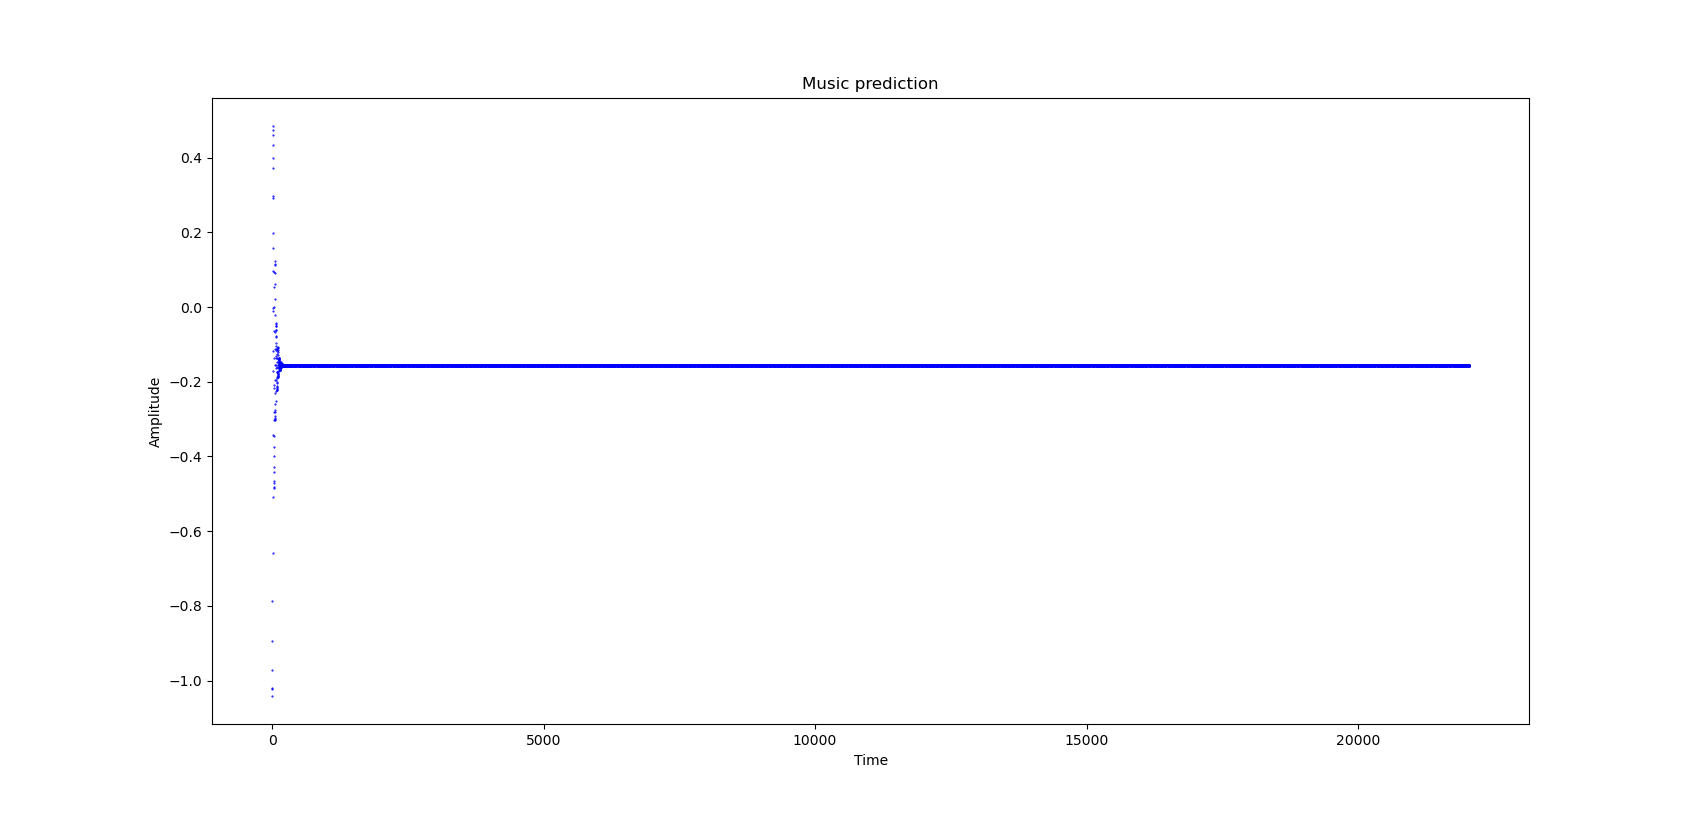
\includegraphics[scale=0.35]{better_convergence.png}
\end{figure}
This is promising as it indicates that music generation is plausible given enough computing power for sufficient training. However in this paper we have limited resources. 
\subsection{Introducing artificial noise}
A possible solution to the convergence of prediction values is to periodically introduce some noise to the prediction process to prevent the model from converging to a stationary value. If we notice a sequence of predictions is too similar we can inject some noise by modifying the prediction seed value at each iteration. 
\begin{figure}[H]
\caption{Prediction figures when we selectively introduce noise to the predicted values to ensure model does not converge to a constant}
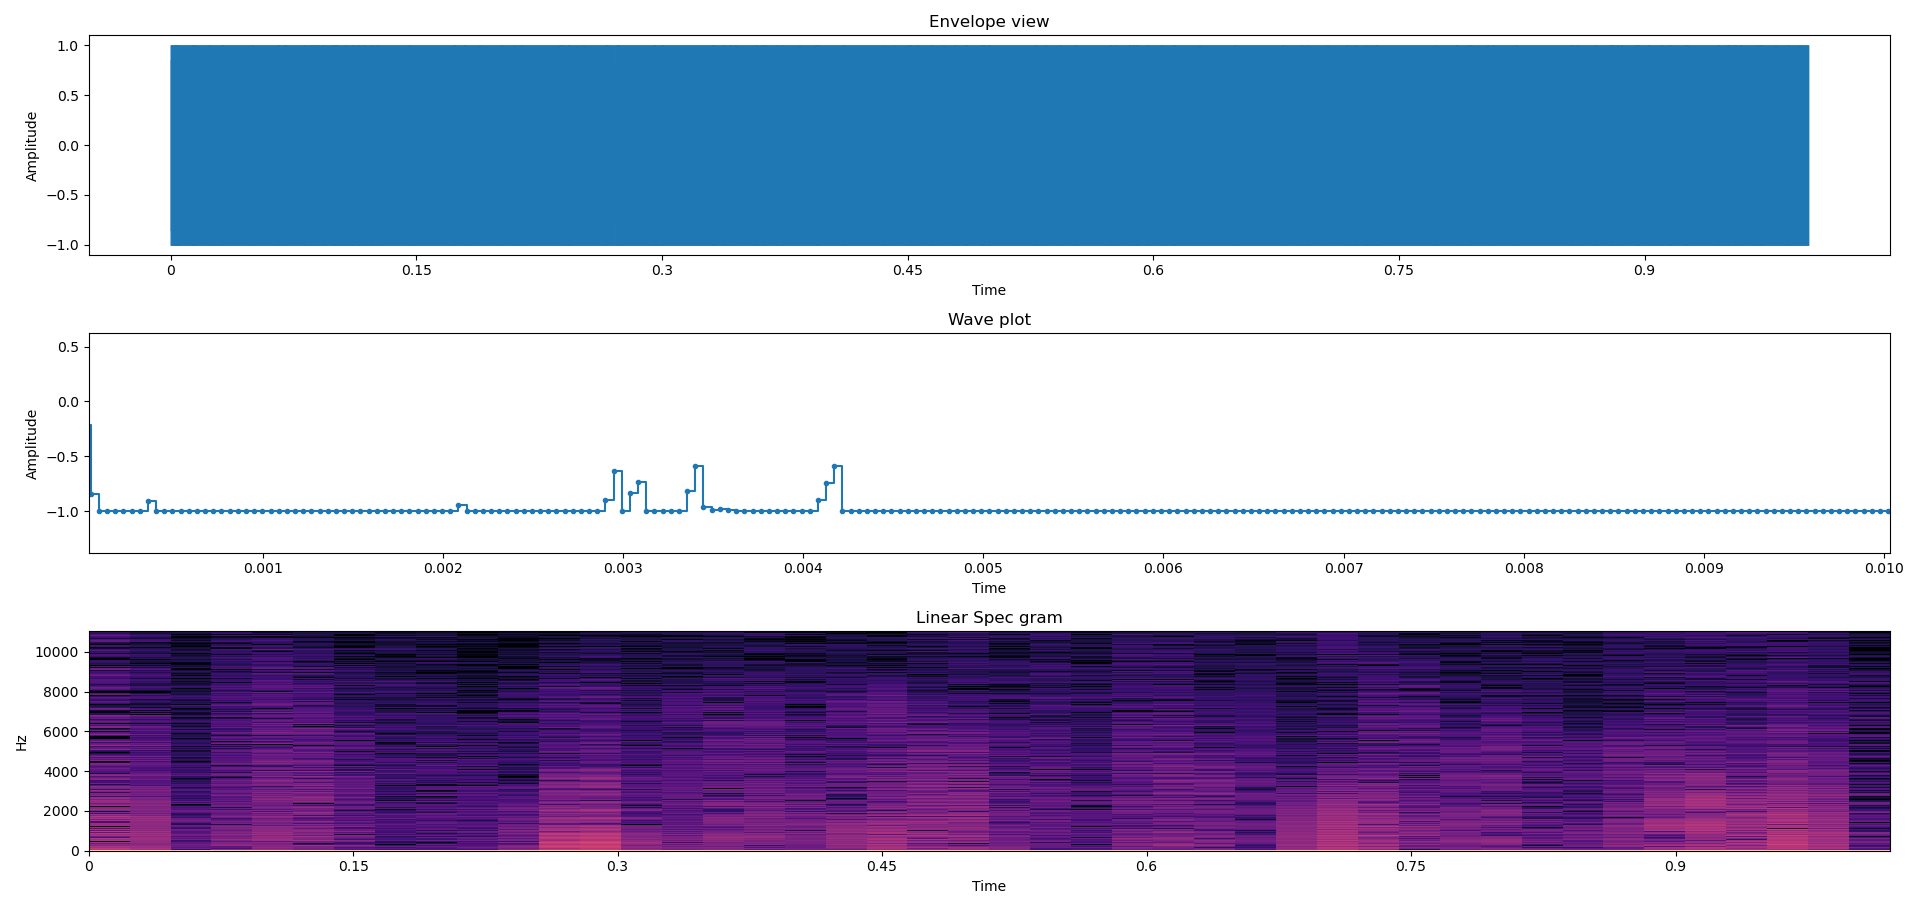
\includegraphics[scale=0.35]{introduction_of_noise.png}
\end{figure}
From the above figure we can see that indeed the scheme does prevent the model from settling for too long on a constant value. However the prediction, qualitatively is just noise, which is evident in the Envelope view. The Wave plot shows us that the noise introduced is low and that the model continuously attempts to move back to the constant. An interesting characteristic of this scheme is the spectrogram shows clear frequency bands indicating some kind of pattern however this pattern does not give rise to any kind of qualitative music. 
\subsection{Predicting from noise}
An interesting investigation that we undertake in this section is rather than using a song as a seed we start prediction with some kind of noise. We will cover two types of noise, normal and perlin. First, the normal noise which is just pseudo random noise that fits a normal distribution. I will not show an input figure for brevity as it is uninteresting. 
\begin{figure}[H]
\caption{Prediction from random normal noise input}
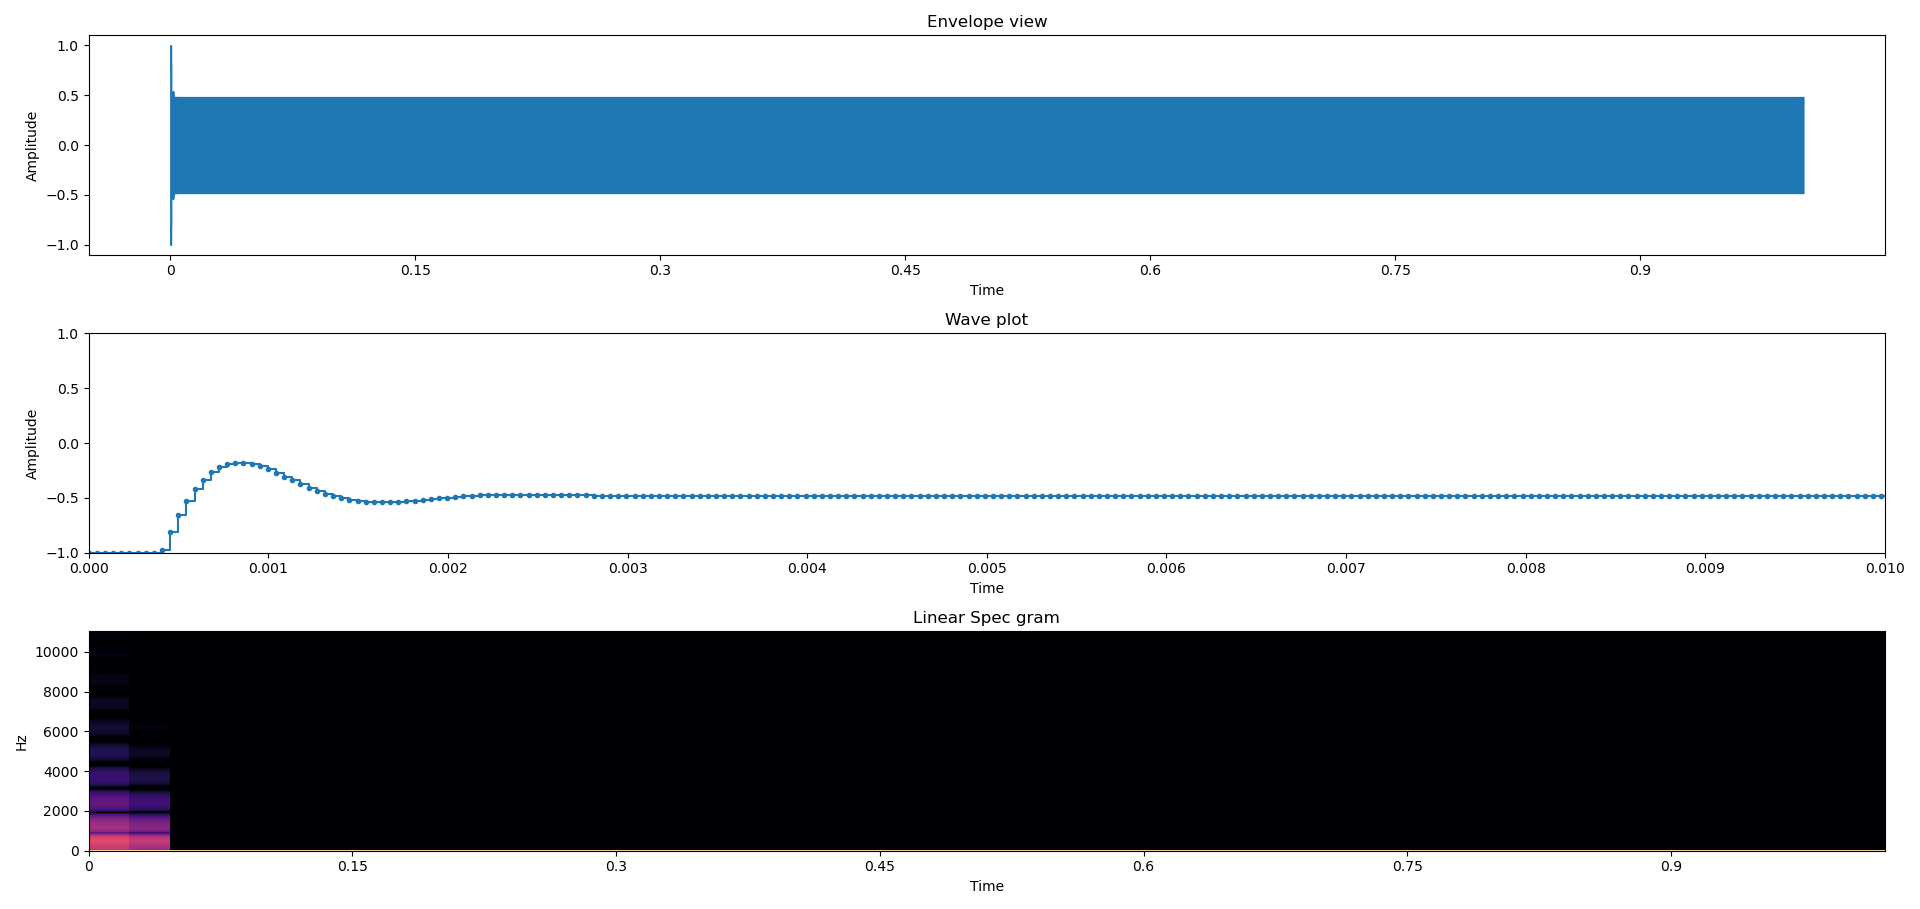
\includegraphics[scale=0.35]{random_normal_prediction.png}
\end{figure}
We see that once again the model produces constant output after some time. But it can be noted that in the time that the model does produce sensible output we can see from the spectrogram that simple noise is produced as output. 
Next we generate results using perlin noise as input. Perlin noise has an almost music like behavior which could lead to interesting results. 
\begin{figure}[H]
\caption{Perlin noise seed}
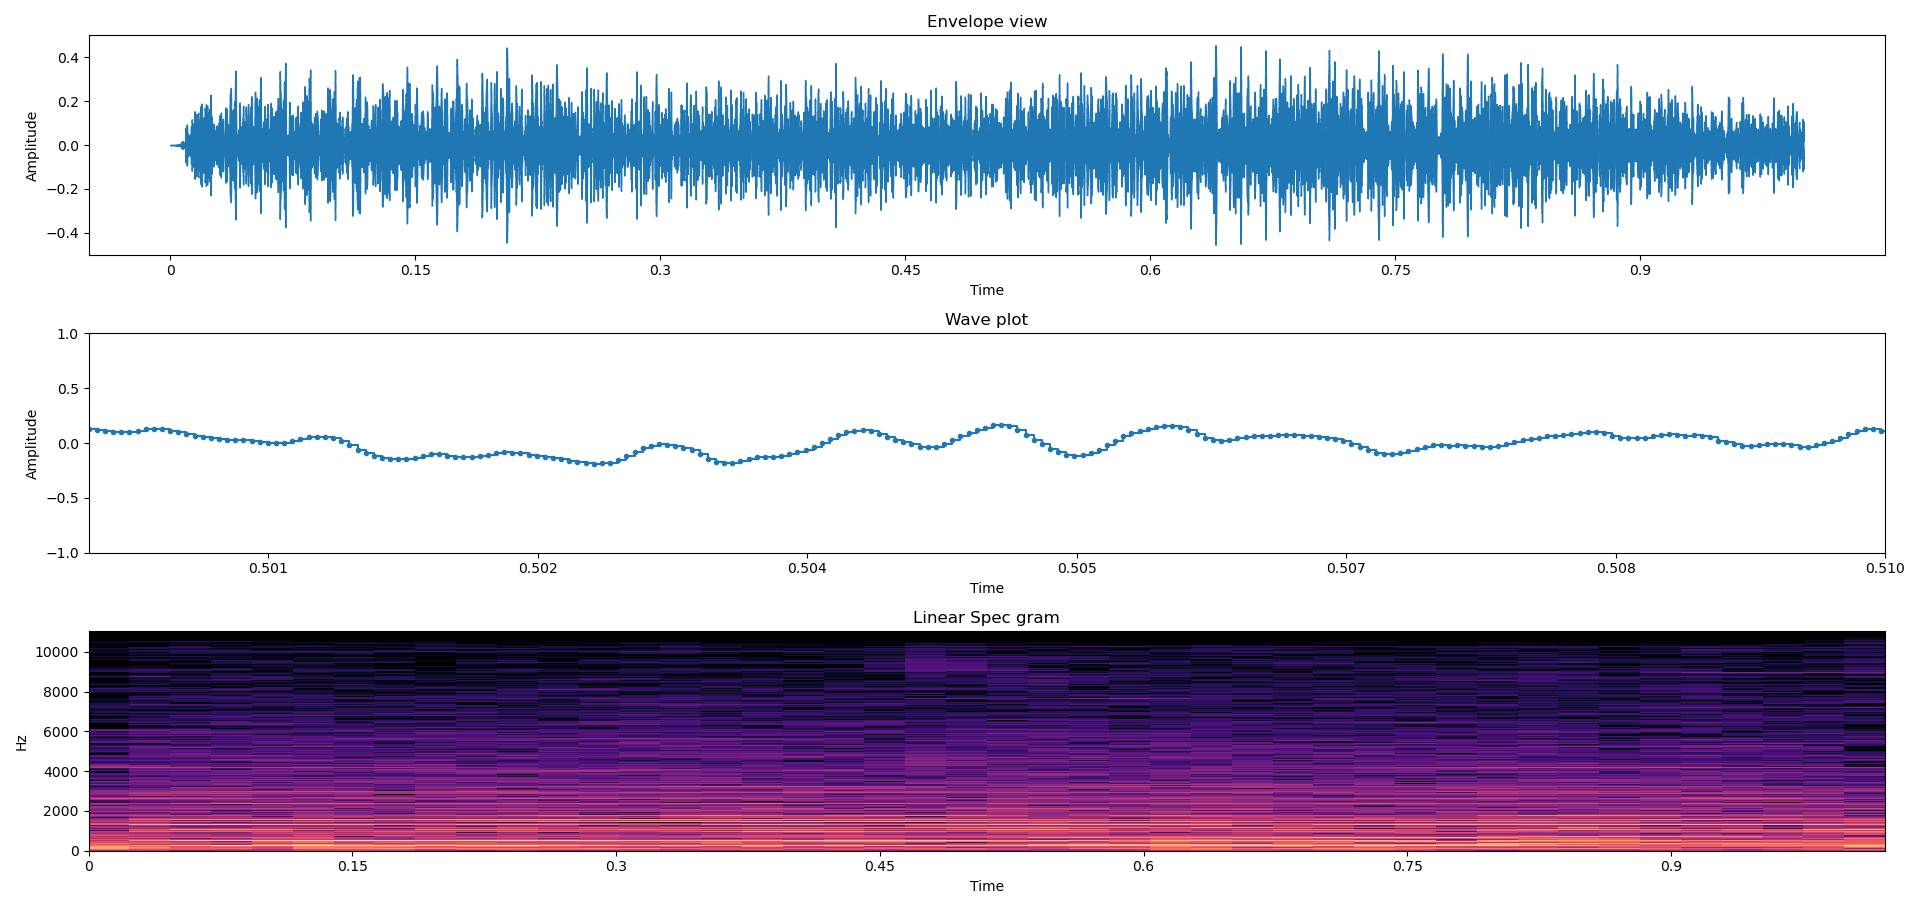
\includegraphics[scale=0.35]{perlin_seed.png}
\end{figure}
\begin{figure}[H]
\caption{Prediction from perlin noise input}
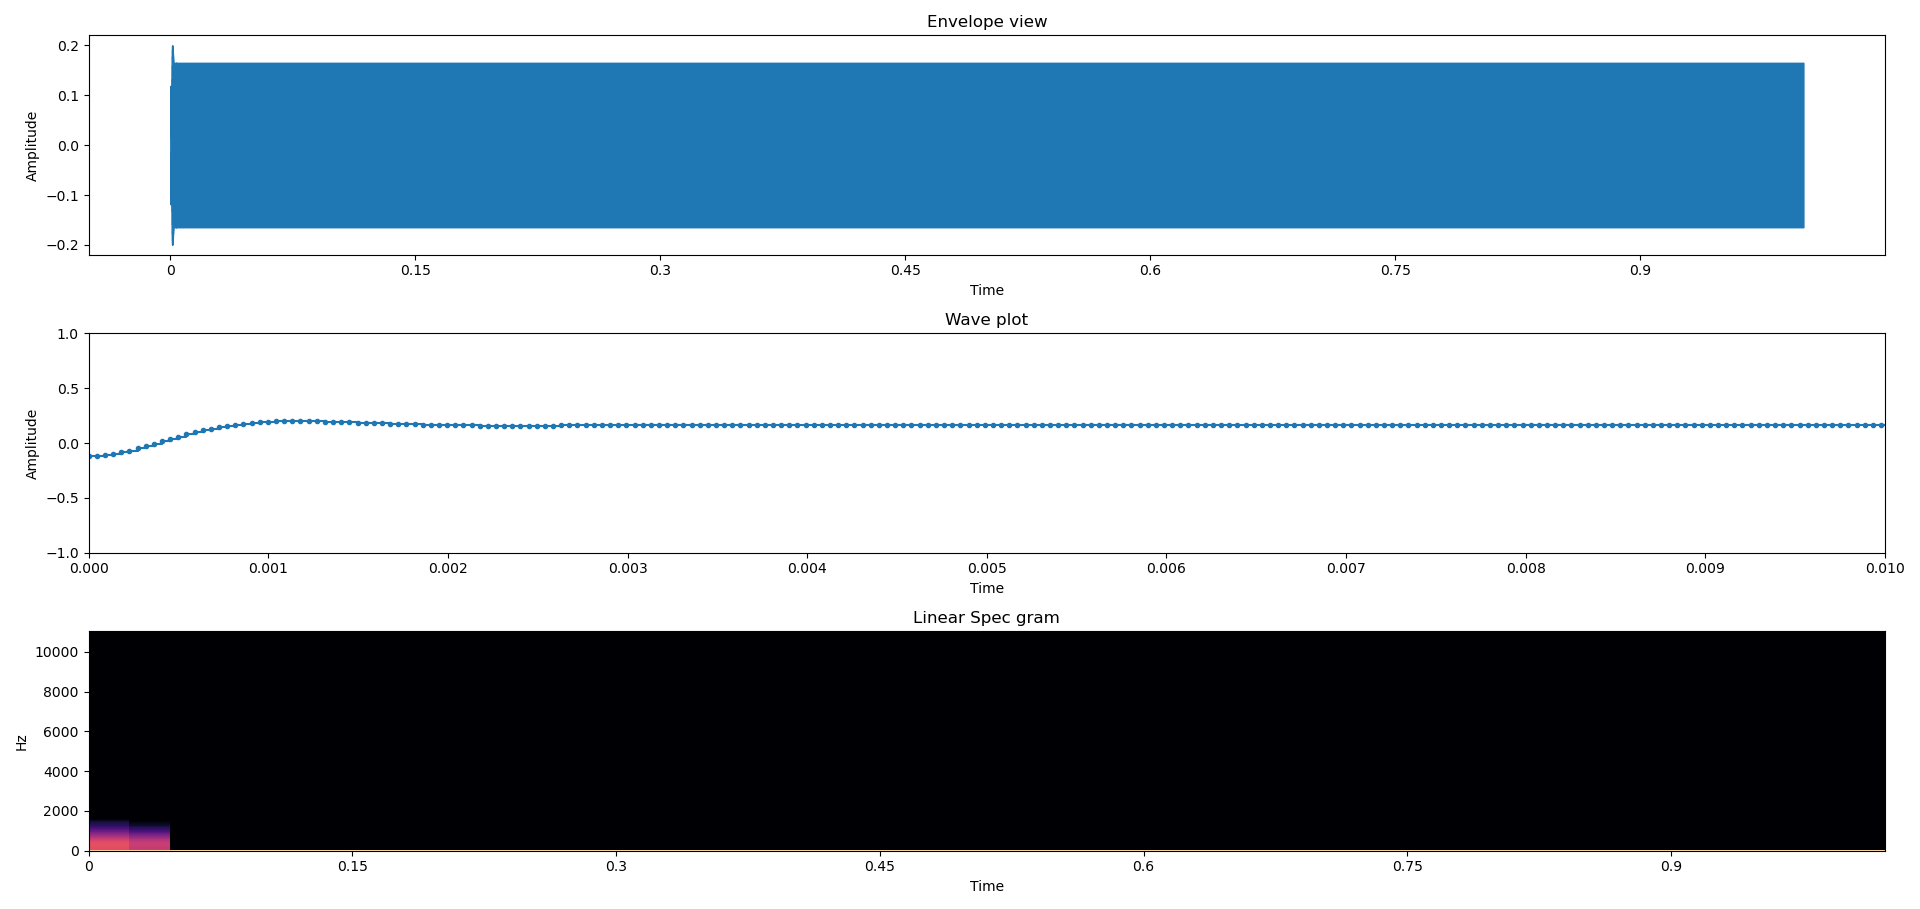
\includegraphics[scale=0.35]{perlin_prediction.png}
\end{figure}
We can once again see that the prediction value converges to a constant. However in this case we can see before the prediction converges a semi stable frequency is created. Reminiscent of the input perlin noise, without complex music behavior. Both of these tests indicate that the model cannot transform any data into a novel music prediction. In order to generate music one must start with a seed that contains the complex behavior of music but not as complex as random data. 
\subsection{Fourier Transform results}
A possible cause of the convergence to a constant predicted value is that the problem is ill phrased. Moreover, the problem is too nonlinear for the size of model to converge on a stable solution. We can rephrase our problem from what is the next to what is the next frequency. This transformation is naturally done by a Fourier Transform of the data. The procedure is as follows use FFT to move to the frequency domain, then scale the data. Train the network on this data. Predict using a starting seed that has been transformed and scaled, then invert the scale and use an ifft scheme to obtain amplitude values that we can write to a sound file. 

In the figure bellow we can see the prediction produced by a model trained on the transformed data. 
\begin{figure}[H]
\caption{Prediction from frequency domain model}
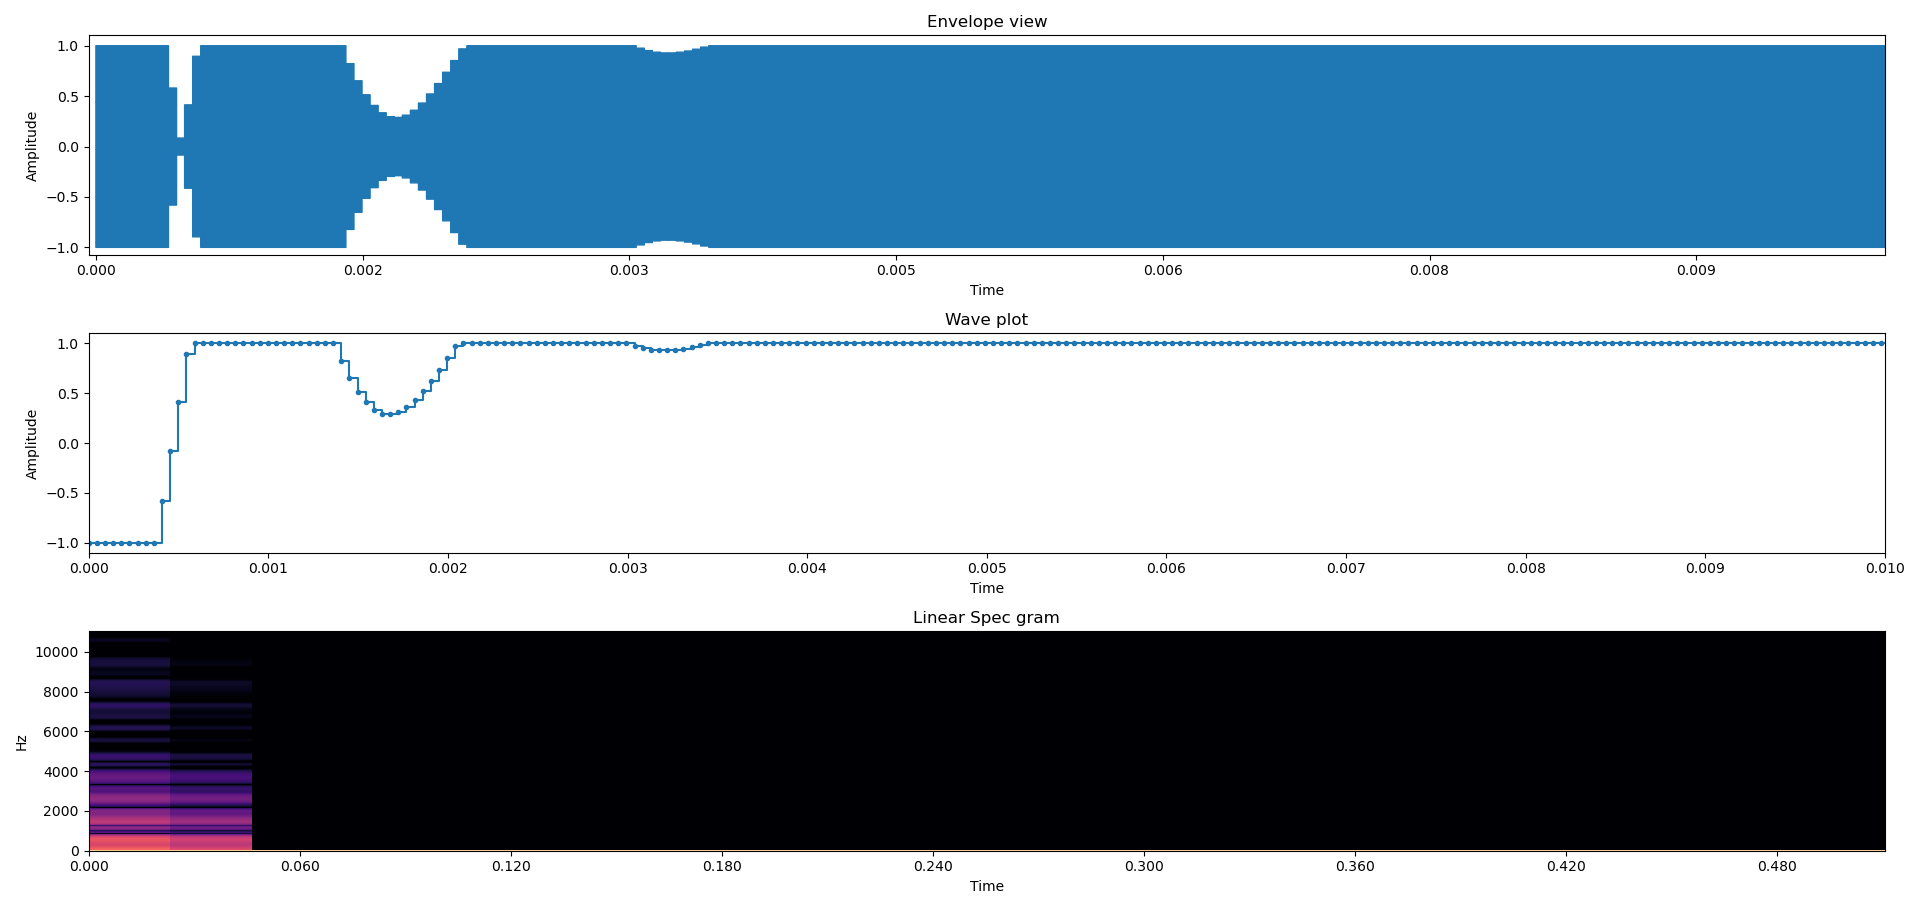
\includegraphics[scale=0.35]{fs_prediction.png}
\end{figure}
As before we see that the model produces a constant output after some time. However, the predictions are valid and appear to be stable for longer than with the amplitude model, the prediction stability lasted for 5\% of the input sequence length. The predictions' interval of stability is too short to make any claims about the sound. But in all the subplots we can see that there is little noise indicating that the frequency domain produces smooth results. It should be noted though that the smoothness of the results does imply that there is little complexity to the predictions and as such the transformation may have dropped some of the higher frequency details that a song may contain.  
\section{Discussion}
In this section I will cover some recommendations for further investigation and discussion of other issues encountered in this work. \\
\subsection{Computational complexity}
Music data in the form of amplitude samples as was covered in this paper leads to massive computational expense as input data can be on the order of hundreds of thousands of elements. Additionally each sample has little effect on the qualitative sound of the music, which necessitates a large and complex model and training scheme. However, for this work I only have access to 32 gigabytes of system memory and 4 gigabytes of GPU memory. The issue of limited system memory was resolved by some memory optimisations, however, the small GPU memory limits the complexity of the model dramatically. In further investigations it would be interesting to see how an RNN like model would perform given a larger computational budget. There was some promising results in this work that indicate, given a longer training sequence one could obtain a model that could reliably generate novel music. 


\subsection{Recommendations for further investigation}
For further investigation:
\begin{enumerate}
\item Attempt music generation with a GRU. In the literature it is well known that the GRU exhibits slightly worse long term memory than the LSTM but has a substantially lower computational cost. 
\item Attempt with more computational power and longer training sequences. 
\item A different data set may yield better or other interesting results.
\item A lossless audio format may be more computationally expensive, but would be interesting to investigate. 
\item Addition of more input features to the model. One could attempt to model a larger input space by extracting more features from an input song. 
\item Using a different model type could be interesting, possibly a convolutional neural network on a spectrogram.
\end{enumerate}
\section{Conclusion}
\label{sec:conclusion}
In this paper we have discussed how to construct and use an LSTM from the principle components used in neural networks. We started with the simplest unit in machine learning, the peceptron and discussed how we can build complex models from this basic unit. We showed the common activation functions that are used in machine learning, how to calculate the loss of a networks output and update the weights accordingly using gradient descent and back propagation. 
\\
We then covered the structure and reasoning behind recurrent models specifically, the standard RNN and LSTM. 
\\
For the practical aspect of this paper we covered the data and prepossessing methods that are useful for the generation of music. This included the dataset used, how digital music is represented and stored, how we can use a Fourier transform to obtain a frequency domain representation of music, the various scaling methods and why we use them. After covering the data  processing we explained the architecture of the NoizeNet model and why it is well suited for novel music generation. \\
The implementation of the model was discussed along with the various hyperparameters that arise during the implementation of a model and their effects. \\
We discussed the stability of our model and how a good choice of learning rate and gradient clipping can ensure that the model remains stable. We explained this works philosophy on batching of data as well as why large sequence lengths are preferable in the scope of this work. \\

In the results section we discussed how to prevent the model from over fitting and demonstrated that NoizeNet was able to learn general knowledge pertaining to music by considering validation loss and training loss graphs. \\
With the knowledge that the model does indeed train effectively we performed an initial test on the model by asking it to reproduce music which it was able to do successfully, all be it with the introduction of some noise. We then compared the performance of an LSTM and RNN where we found that the LSTM exhibits superior modeling qualities but comes with the cost of additional computational resource consumption. \\
We found that when using the model to predict many subsequent values, predictions converged to a constant value and we discussed the possible reasons for this phenomenon. Then we covered the testing used to determine which of the proposed reasons was indeed correct and found that the length of the input sequence was the only parameter that improved the predictive ability of the model. We found that NoizeNet (LSTM) was able to predict novel values for approximately 1\% of the training sequence length. \\
We then proposed that introducing some noise to the prediction values would prevent the convergence of the predictions to a constant value and showed that this proposition was ill founded, in that the model robustly converges to a constant value even under perturbation. \\
We investigated NoizeNets ability to extract musical information from a random prediction seed and found that, although the model has an understanding of music it requires a musical input sequence to model the complex behavior exhibited in music. 
\\
Finally we proposed that NoizeNet would be able to more easily extract musical information from data in a frequency domain and found that indeed the model exhibited better stability, converging to a constant after approximately 5\% of the input sequence length, however, much of the detail in the music was lost during the prediction. 
\\
Overall we found that novel music generation is possible from raw audio formats but requires large input sequences and complex models, both of which were limited by computational resources in this work. 
\printbibliography
\end{document}